% !TeX spellcheck = ru_RU
%pdflatex, utf8
\documentclass[unicode, 10pt, a5paper, oneside]{article}

% Установка полей страницы
%\usepackage{anysize}
%\marginsize{0.3cm}{0.3cm}{0.3cm}{0.3cm}
\usepackage[a5paper, margin=0.3cm, bindingoffset=0cm]{geometry}

% Поддержка русского языка
\usepackage[T2A]{fontenc}		% Корректная кодировка шрифта при использовании cm-super
\usepackage[utf8]{inputenc}		% Кодировка ввода
\usepackage[russian]{babel}		% Словарь расстановки переносов
%\usepackage{cmap}				% Перекодировка символов в pdf при использовании обычного cm

% Всякие математические фишки
\usepackage{amsmath}
\usepackage{amsfonts}
\usepackage{amssymb}

% Изменение цвета, работа с графикой
\usepackage{color}
\usepackage[pdftex]{graphicx}
\graphicspath{{images/}}

% Команда для вставки ссылок \url{URL}
\usepackage[hyphens]{url}
\urlstyle{rm}					% Стиль шрифта ссылок: с засечками

% Кликабельные ссылки внутри документа
\usepackage[unicode]{hyperref}

% Включает отступ у первого абзаца в разделе
\usepackage{indentfirst}

% Настрйока стиля списков
\usepackage{enumitem}
\setlist{noitemsep, leftmargin=*, labelindent=\parindent, topsep=0pt, parsep=0pt, partopsep=0pt}

\setlist[itemize,1]{label=$\diamond$}
\setlist[itemize,2]{label=\textendash}
\setlist[itemize,3]{label=$\star$}

\renewcommand{\alph}[1]{\asbuk{#1}} % Костыль для кирилической нумерации вместо латинской
\setlist[enumerate,1]{label=\arabic*)}
\setlist[enumerate,2]{label=\alph*)}
\setlist[enumerate,3]{label=(\arabic*)}


\usepackage{textcomp}			% Команды для вставки разных символов (градусы, проценты, итд)
\usepackage{float}				% Размещение плавающих объектов там где они созданы (X)
\usepackage{wrapfig}			% Обтекаемые текстом рисунки

% Подписи у флоатов
\setlength{\intextsep}{0pt} % Отстут вокруг плавающих окружений
\usepackage{caption}
\captionsetup{parskip=0pt}
\captionsetup[figure]{labelsep=period,justification=centering,singlelinecheck=false,textfont=small,labelfont=small,aboveskip=2pt,belowskip=0pt}

% Изменение формата заголовков разделов
\usepackage{titlesec}
\titleformat{\section}{\newpage\small\bfseries}{\thesection. }{0pt}{}{}
\titlespacing*{\section}{0pt}{0pt}{0pt}

\titleformat{\subsection}{\small\bfseries}{\thesubsection. }{0pt}{}{}
\titlespacing*{\subsection}{0pt}{0pt}{0pt}

\usepackage{array}				% Позволяет объявить свои типы колонок
\usepackage{calc}				% Математика, исп-ся для расчёта ширины колонки
\usepackage{longtable}			% Длинные таблицы

% Минимальный отступ в таблицах
\setlength{\tabcolsep}{1.5mm}

% Новые типы колонок. Ширина задётся как доля от linewidth
\newcolumntype{L}[1]{p{#1\linewidth-2\tabcolsep-2\arrayrulewidth}}
\newcolumntype{C}[1]{>{\centering}p{#1\linewidth-2\tabcolsep-2\arrayrulewidth}}
\newcolumntype{R}[1]{>{\raggedleft}p{#1\linewidth-2\tabcolsep-2\arrayrulewidth}}
\newcolumntype{U}[2]{p{#1\linewidth-(#2)}}

% Стараться не оставлять одиноких строк в начале и конце абзаца
\clubpenalty=1000
\widowpenalty=1000

% Расстановка отступов и переносов
\emergencystretch=2.5em			% Максимальный промежуток между словами
\tolerance=2000
\frenchspacing


\begin{document}

% Вопрос 1 ----------------------------------------------------------
\section{Полупроводниковые приборы. Классификация. Область применения.}

\subsection*{Виды П/П приборов}

\begin{itemize}
\item Полупроводниковые диоды
\item Полупроводниковые транзисторы
\item Полупроводниковые резисторы
\item Приборы с зарядной связью
\item Полупроводниковые лазеры
\item Оптоэлектронные приборы
\item Микросхемы
\end{itemize}

Принцип работы п/п приборов определяется электронно-дырочным переходом.

Полупроводниковым диодом называется прибор с двумя выводами и одним p-n переходом. Принцип работы полупроводникового диода основан на использовании односторонней проводимости, электрического пробоя и других свойств p-n-перехода. Диоды различают по назначению, материалу, конструктивному исполнению, мощности и другим признакам.

Биполярным транзистором называется полупроводниковый прибор с двумя взаимодействующими p-n переходами. Биполярные транзисторы различаются по структуре. В зависимости от чередования областей различают биполярные транзисторы типа p-n-p и n-p-n.

Полевые транзисторы. Полевым транзистором называется транзистор, в котором между двумя электродами образуется проводящий канал, по которому протекает ток. Управление этим током осуществляется электрическим полем, создаваемым третьим электродом. Электрод, с которого начинается движение носителей заряда, называется истоком, а электрод, к которому они движутся, стоком. Электрод, создающий управляющее электрическое поле, называется затвором. Различают два типа полевых транзисторов: с управляющим p-n переходом и с изолированным затвором (МДП-транзисторы). По типу электропроводности полевые транзисторы подразделяются на транзисторы с каналами p- и n- типов.

Полупроводниковые резисторы нашли широкое применение в электронных приборах. К ним относятся терморезисторы, магниторезисторы, варисторы, фоторезисторы. Принцип действия таких приборов основан на изменении свойств полупроводниковых материалов при воздействии на них температуры, магнитного и электрического полей, электромагнитного излучения.

\subsection*{Классификация П/П приборов}

\begin{enumerate}
\item по технологии изготовления (из кремния, германия, арсенида галлия)
\item по принципу действия:
	\begin{itemize}
	\item диоды: выпрямительные, СВЧ, импульсные, смесительные, стабилитроны, стабисторы. Фотодиоды, светодиоды, тиристоры, динисторы
	\item транзисторы: биполярные, полевые
	\item резисторы: терморезисторы, магниторезисторы, варисторы, фоторезисторы
	\end{itemize}
\end{enumerate}


% Вопрос 2 --------------------------------------------------------
\section{Полупроводниковые диоды. Классификация. Область применения.}

Полупроводниковым диодом называется прибор с двумя выводами и одним p-n переходом. Принцип работы полупроводникового диода основан на использовании односторонней проводимости, электрического пробоя и других свойств p-n-перехода.

В зависимости от технологии изготовления различают точечные диоды, сплавные, микросплавные, эпитаксиальные и другие.

По функциональному назначению диоды делятся на выпрямительные, универсальные, импульсные, смесительные, СВЧ, стабилитроны, стабисторы, варикапы, динисторы, тиристоры, симисторы, фотодиоды, светодиоды и т.д.

По конструктивному исполнению диоды бывают плоскостные и точечные.

По используемому материалу --- кремниевые, германиевые, арсенидгаллиевые. Диоды обладают односторонней проводимостью и служат: для выпрямления переменного тока, стабилизации тока и напряжения, формирования импульсов, для регулирования мощностей и т.д.

Выпрямительные диоды применяются для преобразования переменного тока в постоянный. Они делятся: на маломощные (до 0,3 А), средней мощности (до 1 0А), мощные (более 1000 А), низкочастотные (до 1 кГц) и высокочастотные (до 100 кГц).

Свойства выпрямительных диодов характеризуются вольтамперной характеристикой (ВАХ) и параметрами, которые приводятся в справочной литературе.

\subsection*{Параметры диодов}

\begin{itemize}
\item средний выпрямленный ток Jср
\item прямое падение напряжения Uпр
\item обратный ток диода при заданной температуре Jобр
\item напряжение отсечки Uотс
\item мощность рассеивания Ррас
\item рабочая частота fр. и др.
\end{itemize}

\begin{figure}[H]
\centering
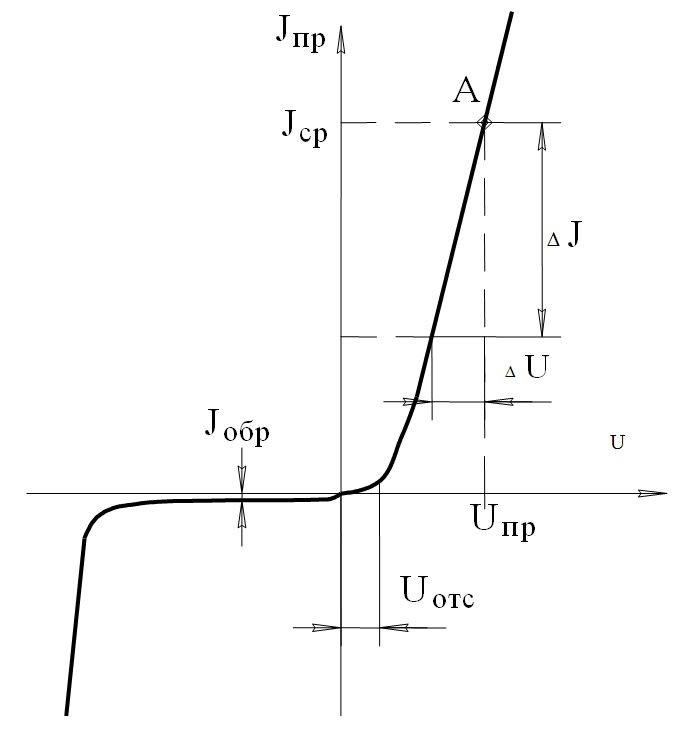
\includegraphics[width=0.4\textwidth]{2_VAC_of_diod.png}
\caption{ВАХ выпрямительного диода}
\label{fig:2_VAC_of_diod}
\end{figure}

\subsection*{Диоды}

Диоды обладают односторонней проводимостью и служат: для выпрямления переменного тока, стабилизации тока и напряжения, формирования импульсов, для регулирования мощностей и т.д.

Выпрямительные диоды применяются для преобразования переменного тока в постоянный. Они делятся: на маломощные (до 0,3А), средней мощности (до 10А), мощные (более 1000А), низкочастотные (до 1кГц) и высокочастотные (до 100кГц).

Свойства выпрямительных диодов характеризуются ВАХ и параметрами, которые приводятся в справочной литературе. Основные параметры диодов: средний выпрямленный ток Jср, прямое падение напряжения Uпр, обратный ток диода при заданной температуре Jобр., напряжение отсечки Uотс., мощность рассеивания Ррас., рабочая частота fр. и др.

\subsection*{Стабилитроны}

Стабилитроны --- это разновидность диодов, предназначенных для стабилизации напряжения. Вольт---амперная характеристика стабилитрона имеет вид. Рабочий участок характеристики АВ лежит в области электрического пробоя диода и характеризуется малым изменением напряжения Uст при значительных изменениях тока.

\begin{figure}[H]
\centering
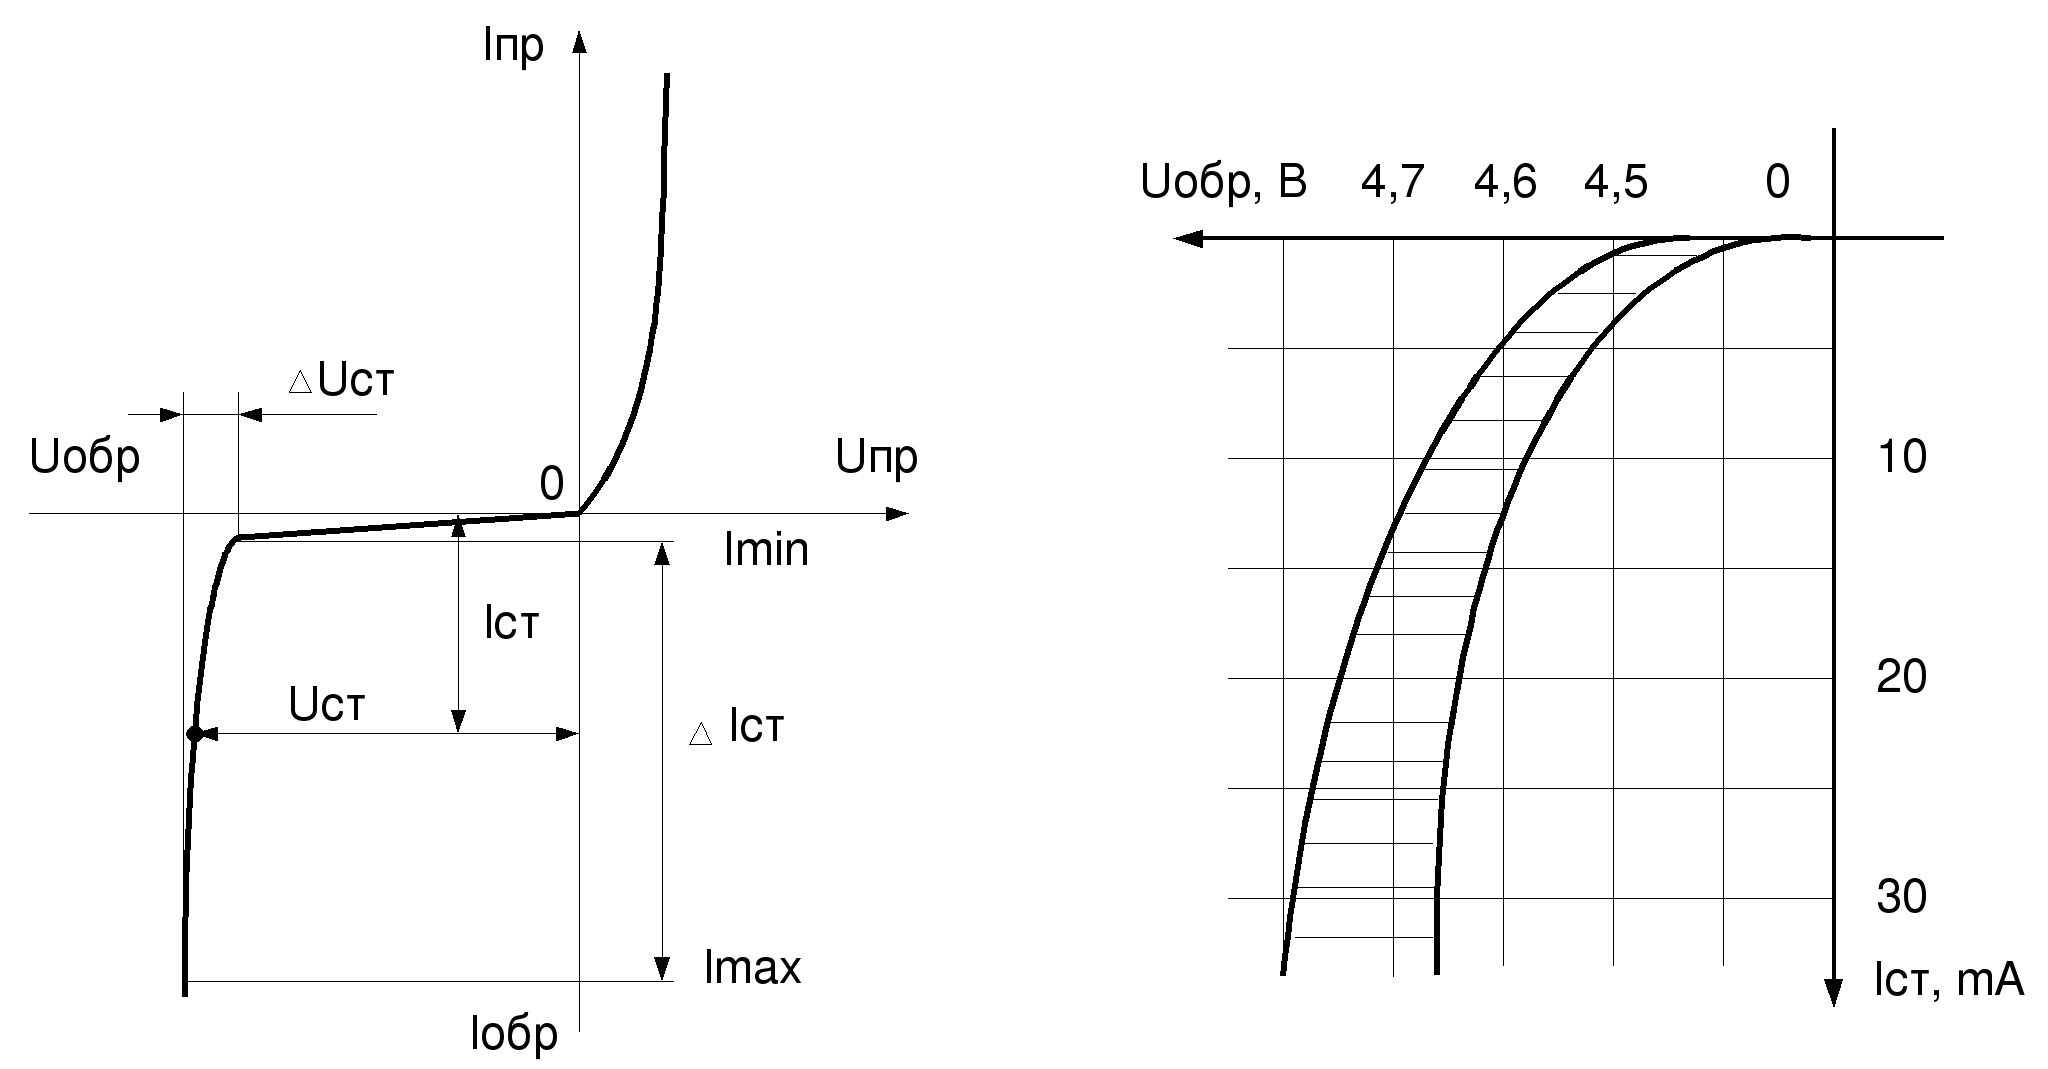
\includegraphics[width=0.7\textwidth]{2_stabilitron.png}
\caption{ВАХ стабилитрона}
\label{fig:2_stabilitron}
\end{figure}

\subsection*{Стабисторы}

Стабисторы, как и стабилитроны, предназначены для стабилизации напряжения. Однако, в отличие от последних, рабочим участком у них является прямая ветвь вольт---амперной характеристики. Стабисторы работают при прямом напряжении и позволяют стабилизировать малые напряжения (0,35 -- 1,9 В).

\begin{figure}[H]
\centering
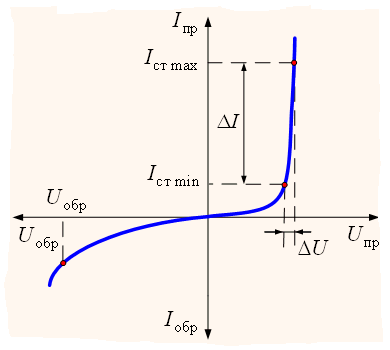
\includegraphics[width=0.5\textwidth]{2_stabistor.png}
\caption{ВАХ стабистора}
\label{fig:2_stabistor}
\end{figure}

\subsection*{Тиристоры, динисторы, симисторы}

Тиристор --- полупроводниковый прибор, выполненный на основе монокристалла полупроводника с тремя или более p-n-переходами и имеющий два устойчивых состояния: закрытое состояние, то есть состояние низкой проводимости, и открытое состояние, то есть состояние высокой проводимости.

Прибор без управляющих электродов называется диодным тиристором или динистором.

\begin{figure}[H]
\centering
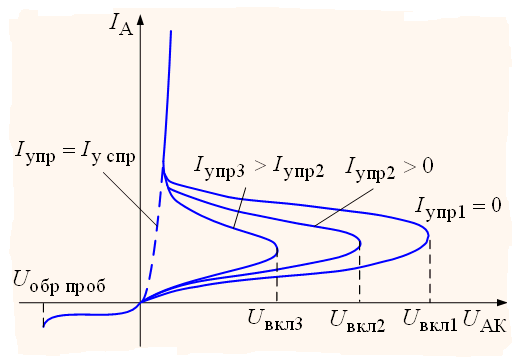
\includegraphics[width=0.5\textwidth]{2_tiristor.png}
\caption{ВАХ тиристора}
\label{fig:2_tiristor}
\end{figure}

Симиcтop (симметричный триодный тиристор) или триак (от англ. TRIAC — triode for alternating current) --- полупроводниковый прибор, являющийся разновидностью тиристоров и используемый для коммутации в цепях переменного тока. В электронике часто рассматривается как управляемый выключатель (ключ). В отличие от тиристора, имеющего катод и анод, основные (силовые) выводы симистора называть катодом или анодом некорректно, так как в силу структуры симистора они являются тем и другим одновременно. Однако по способу включения относительно управляющего электрода основные выводы симистора различаются, причём имеет место их аналогия с катодом и анодом тиристора. На приведённом рисунке верхний по схеме вывод симистора называется выводом 1 или условным катодом, нижний --- выводом 2 или условным анодом, вывод справа --- управляющим электродом.

\subsection*{Варикапы}

Варикап (от англ. vari(able) — «переменный», и cap(acity) — «ёмкость») --- полупроводниковый диод, работа которого основана на зависимости барьерной ёмкости p-n перехода от обратного напряжения. Варикапы применяются в качестве элементов с электрически управляемой ёмкостью в схемах перестройки частоты колебательного контура, деления и умножения частоты, частотной модуляции, управляемых фазовращателей и др.


% Вопрос 3 ------------------------------------------------------------
\section{Полупроводниковые транзисторы. Классификация. Область применения.}

Транзистор --- радиоэлектронный компонент из полупроводникового материала, обычно с тремя выводами, позволяющий входным сигналом управлять током в электрической цепи. Обычно используется для усиления, генерации и преобразования электрических сигналов. В общем случае транзистором называют любое устройство, которое имитирует главное свойство транзистора --- изменения сигнала между двумя различными состояниями при изменении сигнала на управляющем электроде. Далее на схеме приведена классификация.

\subsection*{Классификация транзисторов}

\begin{figure}[H]
\centering
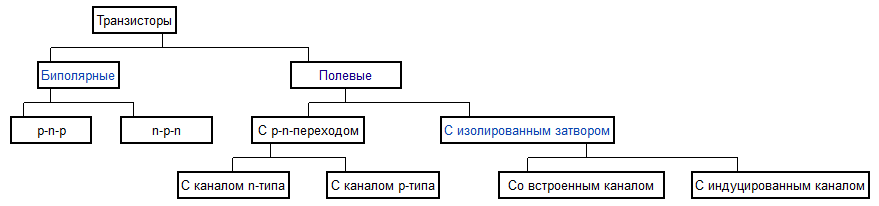
\includegraphics[width=1.0\textwidth]{3_Scheme_of_types.png}
\caption{Классификация транзисторов}
\label{fig:3_Scheme_of_types}
\end{figure}

\subsection*{Биполярный транзистор}

Принцип действия биполярного транзистора основан на использовании физических процессов, происходящих при переносе основных носителей электрических зарядов из эмиттерной области в коллекторную через базу.

$I_\text{э} = I_\text{к} + I_\text{б}$, где $I_\text{э}$, $I_\text{к}$, $I_\text{б}$, --- токи соответственно в цепи эмиттера, коллектора, базы.

\subsection*{Полевой транзистор}

Полевым транзистором называется транзистор, в котором между двумя электродами образуется проводящий канал, по которому протекает ток. Управление этим током осуществляется электрическим полем, создаваемым третьим электродом. Электрод, с которого начинается движение носителей заряда, называется истоком, а электрод, к которому они движутся, стоком. Электрод, создающий управляющее электрическое поле, называется затвором.


% Вопрос 4 ------------------------------------------------------------
\section{Полупроводниковые резисторы. Классификация. Область применения.}

Полупроводниковые резисторы нашли широкое применение в электронных приборах. К ним относятся терморезисторы, магниторезисторы, варисторы, фоторезисторы. Принцип действия таких приборов основан на изменении свойств полупроводниковых материалов при воздействии на них температуры, магнитного и электрического полей, электромагнитного излучения.

Полупроводниковый терморезистор представляет собой прибор, сопротивление которого изменяется при изменении температуры. Зависимость сопротивления от температуры имеет вид:

\begin{equation}
R_{T}=A\exp{\frac{B}{T}}\text{, где}
\end{equation}
\par А, В --- постоянные, определяемые свойствами полупроводникового материала и конструкцией терморезистора;
\par Т --- температура.

С увеличением температуры сопротивление терморезистора уменьшается. Температурный коэффициент сопротивления терморезистора лежит в пределах от 2 до 8,5\% на градус.

Недостатком полупроводниковых терморезисторов является нелинейная зависимость сопротивления от температуры и значительный разброс параметров.

Терморезисторы применяются в качестве первичных преобразователей температуры для контроля и регулирования температуры, а также в схемах температурной компенсации.

Магниторезистор представляет собой полупроводниковый прибор, электрическое сопротивление которого зависит от воздействия на него магнитного поля. Магниторезисторы позволяют обеспечить хорошую гальваническую развязку. Для формирования магнитного поля можно использовать постоянный магнит или электромагнит.

Зависимость сопротивления магниторезистора от величины магнитного поля нелинейна. С увеличением величины магнитного поля сопротивление возрастает.

Основными параметрами магниторезистора являются:

\begin{itemize}
\item ном. сопротивление при отсутствии магнитного поля;
\item мощность рассеивания;
\item ТКR (температурный коэффициент сопротивления);
\item зависимость $R_{B} = f(H)$.
\end{itemize}


\begin{figure}[H]
\centering
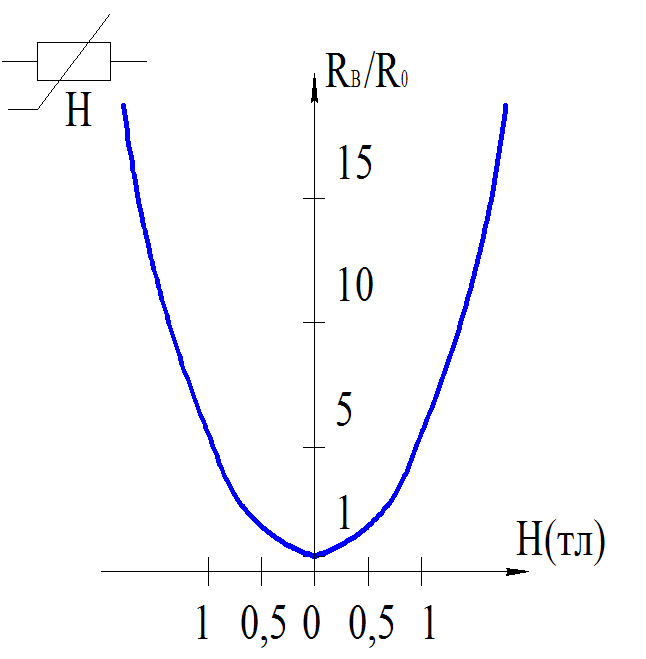
\includegraphics[width=0.35\textwidth]{4_R(H).png}
\hspace{1cm}
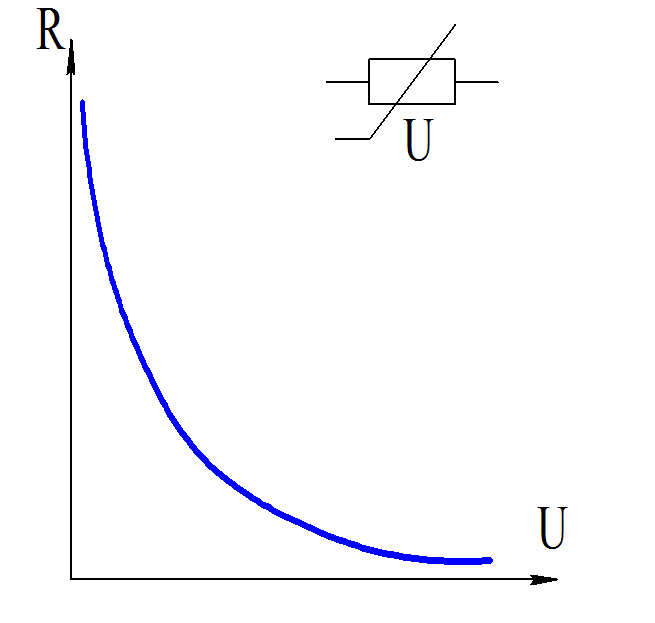
\includegraphics[width=0.35\textwidth]{4_R(U).png}
\\а) \hspace{0.4\textwidth} б)
\caption{Зависимости: R от H (а); R от U (б)}
\label{fig:4_R(U/H)}
\end{figure}

При увеличении магнитной индукции от 0 до 1 Тл сопротивление магниторезистора увеличивается в 10 --- 15 раз. Магниторезисторы нашли применение в коммутационной технике: бесконтактных выключателях, реле, контактах управления. В настоящее время в приборостроении нашли широкое применение магнитодиоды, магнитотранзисторы, магнитотиристоры, которые представляют собой полупроводниковые приборы с p-n-переходами, параметры которых чувствительны к магнитному полю.

Варисторы представляют собой полупроводниковые резисторы, сопротивление которых зависит от приложенного напряжения. Зависимость сопротивления от напряжения нелинейная. Сопротивление RВ уменьшается при увеличении приложенного напряжения. Варисторы применяются для защиты от перенапряжений, защиты от помех, для искрогашения в электрических машинах. Они ограничивают возникающее напряжение, особенно при коммутации индуктивной или емкостной нагрузки и тем самым позволяют значительно повысить срок службы контактов реле и т.д.

Фоторезисторы представляют собой полупроводниковые приборы, сопротивление которых зависит от электромагнит. излучения.


% Вопрос 5 ----------------------------------------------------------
\section{Фотоэлектрические приборы. Классификация. Область применения.}

Фотоэлектрические приборы строятся на принципах фотопроводимости.

Фотопроводимость --- это свойство веществ изменять свою электропроводность под воздействием электромагнитного излучения.

\subsection*{Классификация фотоэлектронных приборов}

\begin{enumerate}
\item с внешним фотоэффектом
	\begin{itemize}
	\item вакуумные
	\item газонаполненные фотоэлементы (ФЭ)
	\item фотоэлектронные умножители (ФЭУ)
	\end{itemize}
\item с внутренним фотоэффектом
	\begin{itemize}
	\item фоторезисторы
	\item фотодиоды
	\item фототранзисторы
	\item фототиристоры
	\end{itemize}
\end{enumerate}

В качестве излучателей используется солнечный свет, лампочки накаливания и другие источники света.

Фотоэлемент (ФЭ) --- это электровакуумный или газоразрядный диод, в стеклянном баллоне которого установлены фотокатод и фотоанод. Фотокатод представляет собой слой, покрывающий внутреннюю поверхность колбы, выполненный из полупроводникового материала, чувствительного к внешнему излучению. Анод выполнен в виде кольца или рамки и размещен внутри колбы. ФЭ разделяются на вакуумные и газоразрядные.

При отсутствии излучения анодный ток равен нулю. При освещении фотокатода возникает фотоэмиссия, и в цепи анода протекает ток.

Фотоэлементы используются в первичных преобразователях информации.

\subsection*{Фотоэлектронный умножитель}

Фотоэлектронный умножитель представляет собой электровакуумный прибор, преобразующий энергию электромагнитного излучения в электрические сигналы с использованием вторичной электронной эмиссии. Состоит из стеклянного баллона, внутри которого расположены ускоряющие электроды, умножительные электроды и анод. При освещении фотокатода возникает электронный поток, который фокусируется и направляется на умножительные электроды, где за счет вторичной эмиссии он усиливается и попадает на анод.

\begin{figure}[H]
\centering
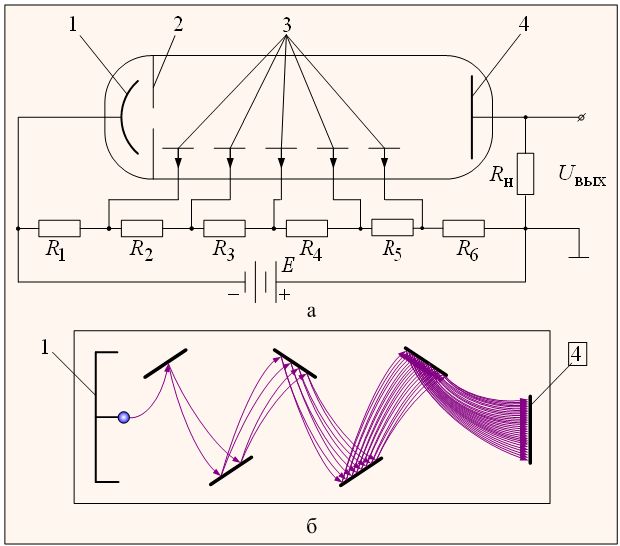
\includegraphics[width=0.65\textwidth]{5_PEM.png}
\caption{Фотоэлектронный умножитель}
\label{fig:5_PEM}
\end{figure}

\subsection*{Фоторезистор}

Фоторезистор представляет собой полупроводниковый прибор, сопротивление которого зависит от освещенности.

\subsection*{Фотодиод}

Фотодиод представляет собой полупроводниковый прибор с n-p переходом. Принцип работы фотодиода заключается в том, что при его освещении возрастает обратный ток, и он не зависит от обратного напряжения. На границе перехода “n-p” возникает ЭДС, величина которой зависит от освещенности и может достигать 0,5 --- 1 В. При этом обратное сопротивление фотодиода уменьшается.

Они относятся к быстродействующим приборам и реагируют на сигналы до 1 МГц. Фотодиоды могут также использоваться в качестве источников питания, например, в солнечных батареях.

\subsection*{Фототранзистор}

Фототранзистор в отличие от фотодиода является активным преобразователем, в нем происходит не только преобразование энергии излучения, но и усиление.

Внутренний фотоэффект в полупроводнике может быть использован для построения других приборов, например, фототиристоров, однопереходных фототранзисторов и др.

\begin{figure}[H]
\centering
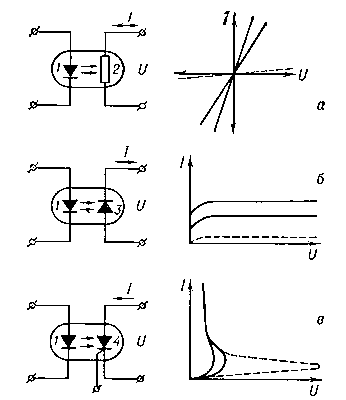
\includegraphics[width=0.5\textwidth]{5_ptiristor.png}
\caption{УГО и ВАХ фотоэлементов}
\label{fig:5_ptiristor}
\end{figure}


% Вопрос 6 ----------------------------------------------------------------------
\section{Аналоговые усилители. Классификация. Основные характеристики и параметры.}

Усилитель --- устройство, предназначенное для усиления электрических сигналов по напряжению, току или мощности за счет преобразования энергии источника питания в энергию выходного сигнала. Усилитель включает в себя нелинейный элемент, управляемый входным электрическим сигналом $U_\text{вх}$, источник питания $U_\text{п}$ и нагрузочное устройство с сопротивлением $Z_\text{н}$. Аналоговые усилители служат для усиления аналоговых сигналов.

\subsection*{Классификация усилителей}

\begin{itemize}
\item по виду усиливаемого:
	\begin{itemize}
	\item гармонических сигналов
	\item импульсных сигналов
	\end{itemize}
\item по типу усиливаемого сигнала:
	\begin{itemize}
	\item напряжения
	\item тока 
	\item мощности
	\end{itemize}
\item по диапазону усиливаемых частот:
	\begin{itemize}
	\item постоянного тока 
	\item переменного тока. Которые в зависимости от диапазона усиливаемых частот делятся на:
		\begin{itemize}
		\item усилители низкой частоты (УНЧ)
		\item высокой частоты (УВЧ)
		\item широкополосные
		\item избирательные усилители.
		\end{itemize}
	\end{itemize}
\item по виду нагрузки:
	\begin{itemize}
	\item с активной нагрузкой
	\item c активно-индуктивной нагрузкой
	\item c емкостной нагрузкой
	\end{itemize}
\item по количеству каскадов:
	\begin{itemize}
	\item однокаскадные 
	\item многокаскадные. Связь в между каскадами может быть:
		\begin{itemize}
		\item гальванической
		\item емкостной
		\item индуктивной
		\end{itemize}
	\end{itemize}
\end{itemize}

\subsection*{Основные характеристики усилителя}

\begin{itemize}
\item амплитудная характеристика, которая представляет собой зависимость $U_\text{выx} = \varphi(U_\text{вх})$. Для линейных усилителей это прямая, проходящая через начало координат;
\item амплитудно-частотная характеристика (АЧХ) $U_\text{выx} = \varphi(f)$ отражает зависимость амплитуды выходного сигнала от частоты. Реально в усилителях из-за наличия паразитных емкостей и индуктивностей различные частоты усиливаются неодинаково;
\item фазо-частотная характеристика $U_\text{выx} = \lambda(f)$ отражает зависимость угла сдвига фазы выходного сигнала по отношению к фазе входного сигнала;
\item переходная характеристика --- отражает реакцию усилителя на единичный скачок входного напряжения. Переходная характеристика определяется по ее изображению на экране осциллографа при подаче на вход усилителя входного сигнала прямоугольной формы. Процесс изменения выходного сигнала может быть колебательным либо апериодичным.
\end{itemize}

\subsection*{Важнейшие параметры усилителя}

\begin{itemize}
\item коэффициент усиления по току $K_{I} = \dfrac{\Delta I_\text{вых}}{\Delta I_\text{вх}}$
\item коэффициент усиления по напряжению $K_{U} = \dfrac{\Delta U_\text{вых}}{\Delta U_\text{вх}}$
\item коэффициент усиления по мощности $K_{P} = \dfrac{\Delta P_\text{вых}}{\Delta P_\text{вх}}$
\item Полоса пропускания усилителя $2\Delta f$ характеризует частотные свойства усилителя. Измеряется на уровне $0,707 K_{max}$
\end{itemize}

Для наглядности в ряде случаев АЧХ строится в относительных единицах усиления.
\begin{equation}
N(F) = \dfrac{K(f)}{K_{max}}\text{, где}
\end{equation}
\par $K(f)$ --- коэффициент усиления на частоте $f$;
\par $K_{max}$ --- максимальный коэффициент усиления.

Входное и выходное сопротивление необходимо учитывать при согласовании с источником входного сигнала и с нагрузкой. 

Выходная мощность усилителя --- это мощность, которая выделяется на нагрузке.

Искажения сигналов в усилителе --- это отклонение формы выходного сигнала от формы входного сигнала. Различают два вида искажений: статические (нелинейные) и динамические (линейные). Нелинейные искажения возникают в усилителе за счет работы его на нелинейном участке ВАХ. Количественно нелинейные искажения оцениваются коэффициентом нелинейных искажений.

\begin{equation}
K_{H} = \dfrac{\sqrt{(A_{2}^{2} + A_{3}^{2} + \ldots + A_{n}^{2})} }{A_{1}}\text{, где}
\end{equation}
\par $A_{n}$ --- амплитуда n-й гармоники;
\par $A_{1}$ --- амплитуда основной гармоники выходного сигнала.

Линейные искажения определяются амплитудно-частотной характеристикой усилителя и количественно оцениваются коэффициентами частотных искажений на низких и высоких частотах.

Для получения высоких коэффициентов усиления в состав усилителя входит обычно несколько каскадов. Первым каскадом, как правило, является предварительный усилитель, затем идут промежуточный усилитель и усилитель мощности. Предварительный усилитель обеспечивает связь источника сигнала с усилителем. Он должен иметь большое входное сопротивление для того, чтобы не ослаблять входной сигнал. Промежуточный усилитель обеспечивает основное усиление, а усилитель мощности обеспечивает заданную выходную мощность.

При построении усилительных устройств наибольшее распространение получили каскады на биполярных и полевых транзисторах, включенных с ОЭ (OU) или с ОК (OC).

% Вопрос 7 -----------------------------------------------------------------------------------------
\section{Избирательные усилители. Усилители постоянного тока. Усилители мощности. Область применения.}

Избирательными называются усилители, усиливающие сигналы в относительно узкой полосе частот. Основными показателями избирательных усилителей являются максимальный коэффициент усиления, полоса пропускания, средняя частота полосы пропускания и избирательность. Основным требованием, предъявляемым к избирательным усилителям, является получение высокой избирательности, которая определяется крутизной склонов его амплитудно-частотной характеристики. Чем круче спады частотной характеристики и чем меньше коэффициент усиления усилителя за пределами полосы пропускания, тем выше его избирательность. Избирательность таких усилителей оценивают величиной коэффициента прямоугольности АЧХ, который равен отношению ширины полосы пропускания на уровне 0,7 к ширине полосы на уровне 0,1 (или к ширине полосы на уровне 0,01):

\begin{equation}
K_\text{п} = \dfrac{2\Delta f_{0,7}}{2\Delta f_{0,01 - 0,1}}
\end{equation}

Избирательные усилители применяются в основном для усиления сигналов высокой частоты и разделяются на два вида: резонансные усилители и полосовые усилители. В резонансных усилителях нагрузкой обычно является одиночный параллельный колебательный контур. Перестраивая контур, можно изменять резонансную частоту в некоторых пределах.

Полосовые усилители обеспечивают амплитудно-частотную характеристику по форме близкую к прямоугольной. Полосовые усилители не перестраиваются и работают на фиксированных частотах. В качестве нагрузки они имеют один или два колебательных контура в каждом каскаде. В усилителях промежуточной частоты радиоприемников применяются также фильтры сосредоточенной селекции, состоящие из трех-четырех связанных колебательных контуров. В качестве фильтров сосредоточенной селекции также широко применяются пьезоэлектрические фильтры. В них благодаря прямому и обратному пьезоэлектрическому эффекту амплитудно-частотная характеристика формируется в системе из нескольких механических резонаторов.

Однокаскадный резонансный усилитель состоит из активного элемента, нагрузкой которого является одиночный параллельный колебательный контур. В качестве активного элемента можно использовать биполярные или полевые транзисторы, включаемые, чаще всего, по схеме с общим эмиттером или общим истоком. При этом колебательный контур оказывается зашунтированным выходным сопротивлением собственного каскада и входным сопротивлением следующего каскада в многокаскадном усилителе, за счет чего избирательность ухудшается. В каскадах с полевым транзистором колебательный контур шунтируется слабо, так как входное и выходное сопротивление полевого транзистора достаточно большое. В таких каскадах возможно полное включение контура в нагрузочную цепь. Биполярные транзисторы имеют относительно малые значения входных и выходных сопротивлений. Поэтому при непосредственном включении колебательного контура в нагрузочную цепь контур шунтируется значительно сильнее и его избирательные свойства заметно ухудшаются. Поэтому в резонансных 
каскадах на биполярных транзисторах принимают специальные меры для уменьшения шунтирующего действия входного и выходного сопротивления транзистора. С этой целью ослабляют связь транзистора с колебательным контуром, используя частичное включение контура в нагрузочную цепь. В связи с тем, что резонансные избирательные усилители работают на высокой частоте, существенное влияние на их работу может оказывать внутренняя обратная связь, имеющаяся между входом и выходом в любом активном элементе. Эта внутренняя обратная связь на одной из высоких частот может оказаться положительной, что приведет к нарушению устойчивой работы усилителя и его самовозбуждению. Для повышения устойчивости работы каскада необходимо ослаблять связь его активного элемента с колебательным контуром. С этой целью частичное включение контура используют и в резонансных каскадах на полевых транзисторах. Далее на рисунке показана схема резонансного усилителя на полевом транзисторе с полным включением контура и его АЧХ.

\subsection*{Схема на полевом транзисторе}

Модуль коэффициента усиления каскада на полевом транзисторе при полном включении контура примерно равен:

\begin{equation}
|K_\text{рез}| \approx S R_\text{рез}
\end{equation}
где $ R_\text{рез} = Q\rho $ --- сопротивление параллельного контура на резонансной частоте.

\begin{figure}[H]
\centering
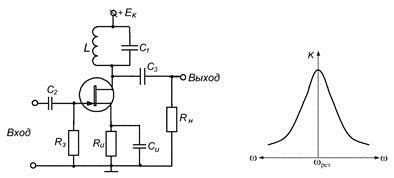
\includegraphics[width=0.6\textwidth]{7_field_based_amp.jpg}
\caption{Избирательный усилитель на полевом транзисторе и его АЧХ}
\label{fig:7_field_based_amp}
\end{figure}

\subsection*{Схема на биполярном транзисторе}

Далее показана схема избирательного усилителя на биполярном транзисторе с неполным включением контура. Для каскада на биполярном транзисторе при неполном включении контура в цепь нагрузки необходимо учитывать коэффициенты подключения контура и модуль коэффициента усиления будет определяться следующим выражением:

\begin{equation}
|K_\text{рез}| = b_{1}b_{2} \dfrac{\beta R_\text{рез}}{R_\text{вх}}
\end{equation}
где $ b_{1} = \dfrac{L\prime}{L} $ и $ b_{2} = \dfrac{L\prime\prime}{L} $ --- коэффициенты включения контура; $L$ --- полная индуктивность катушки; $L\prime$ --- индуктивность части катушки, к которой подключен коллектор транзистора; $L\prime\prime$ --- индуктивность части катушки, с которой усиленный сигнал снимается на вход следующего каскада.

\begin{figure}[H]
\centering
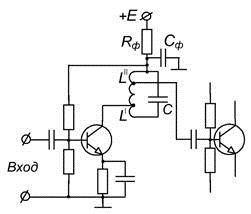
\includegraphics[width=0.4\textwidth]{7_bipolar_based_amp.jpg}
\caption{Избирательный усилитель на биполярном транзисторе}
\label{fig:7_bipolar_based_amp}
\end{figure}

\subsection*{2T-мост}

При необходимости избирательного усиления низких частот емкости и индуктивности колебательного контура должны быть большими и добротность контура оказывается низкой при значительном увеличении габаритов катушки и конденсатора. Поэтому в качестве низкочастотных избирательных усилителей используют усилители с частотно-зависимой отрицательной обратной связью. В качестве частотно-зависимой цепи используют двойной T-образный мост (2T-мост).

\begin{figure}[H]
\centering
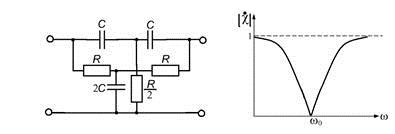
\includegraphics[width=0.6\textwidth]{7_2T.jpg}
\caption{Схема 2T-моста и АХЧ}
\label{fig:7_2T}
\end{figure}

Если включить 2T-мост в цепь отрицательной обратной связи в RC-усилитель, то поскольку на частоте $\omega = \omega_{0}$ коэффициент передачи моста равен нулю, отрицательная обратная связь будет отсутствовать, и коэффициент усиления усилителя будет максимальным. На всех остальных частотах коэффициент усиления избирательно уменьшается из-за наличия отрицательной обратной связи. В результате амплитудно-частотная характеристика усилителя с 2T-мостом в цепи отрицательной обратной связи будет иметь ярко выраженный максимум на частоте $\omega_{0}$.

\begin{figure}[H]
\centering
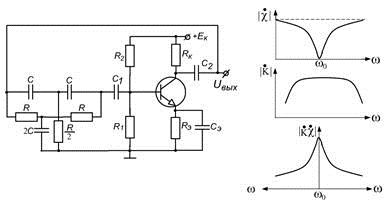
\includegraphics[width=0.6\textwidth]{7_2T_with_feedback.jpg}
\caption{Схема 2T-моста с обратной связью и АХЧ}
\label{fig:7_2T_with_feedback}
\end{figure}

Схема избирательного усилителя с 2T-мостом эквивалентна резонансному каскаду, имеющему добротность $Q = \dfrac{K}{4}$ , где $K$- коэффициент усиления усилителя без обратной связи. Для увеличения эквивалентной добротности избирательной системы можно цепью отрицательной обратной связи через 2Т-мост охватывать несколько каскадов усиления.

\subsection*{Усилители постоянного тока}

Усилителями постоянного тока называют такие устройства, которые могут усиливать медленно изменяющиеся электрические сигналы, то есть они способны усиливать и переменные и постоянные составляющие входного сигнала. Усилители постоянного тока имеют много разновидностей (дифференциальные, операционные, усилители с преобразованием входного сигнала и др.). Поскольку такие устройства пропускают наряду с переменной составляющей еще и постоянную, то отдельные каскады должны быть связаны между собой либо непосредственно, либо через резисторы, но не через разделительные конденсаторы или трансформаторы, которые не пропускают постоянную составляющую. Основную проблему усилителей постоянного тока представляет дрейф нуля --- отклонение напряжения на выходе усилителя от начального (нулевого) значения при отсутствии входного сигнала. Основной причиной этого явления являются температурная и временная нестабильность параметров активных элементов схемы усилителя, резисторов, а также источников питания. Одним из возможных путей 
уменьшения дрейфа нуля является использование дифференциальных усилителей.

\begin{itemize}
\item Дифференциальные усилители предназначены для усиления сколь угодно медленно изменяющихся во времени сигналов, частотный диапазон которых начинается от 0 Гц.
\item Дифференциальный усилитель: имеет следующие достоинства: малый дрейф нуля; высокая степень подавления синфазных помех.
\item Недостатки дифференциального усилителя: требует двухполярного источника питания; необходима очень высокая симметрия схемы.
\end{itemize}

\begin{figure}[H]
\centering
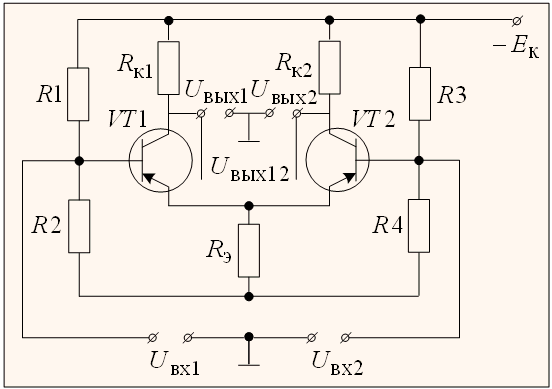
\includegraphics[width=0.5\textwidth]{7_diff_amp.png}
\caption{Схема простейшего дифференциального усилителя}
\label{fig:7_diff_amp}
\end{figure}

\begin{itemize}
\item Дифференциальные усилители предназначены для усиления сколь угодно медленно изменяющихся во времени сигналов, частотный диапазон которых начинается от 0 Гц.
\item Дифференциальный усилитель: имеет следующие достоинства: малый дрейф нуля; высокая степень подавления синфазных помех.
\item Недостатки дифференциального усилителя: требует двухполярного источника питания; необходима очень высокая симметрия схемы.
\end{itemize}


% Вопрос 8 ------------------------------------------------------------------------
\section{Операционные усилители. Классификация. Область применения. Балансировка ОУ.}

Операционным усилителем называют усилитель постоянного тока, предназначенный для выполнения различного рода операций над аналоговыми сигнала при работе в схемах с отрицательной обратной связью.

Операционные усилители обладают большим и стабильным коэффициентом усиления напряжения, имеют дифференциальный вход с высоким входным сопротивлением и несимметричный выход с низким выходным сопротивлением, малым дрейфом нуля. То есть под операционным усилителем понимают высококачественный универсальный усилитель.

Условные обозначения операционных усилителей приведены ниже. Один из входов, обозначенный знаком «+» называют неинвертирующим (прямым), так как сигнал на выходе и сигнал на этом входе имеют одинаковую полярность. Второй вход, обозначенный знаком «-», (его также обозначают знаком инверсии «o») называют инвертирующим, так как сигнал на выходе по отношению к сигналу на этом входе имеет противоположную полярность. Помимо трех сигнальных контактов (двух входных и одного выходного) операционный усилитель содержит дополнительные контакты (обычно число контактов составляет 14 или 16).

\begin{figure}[H]
\centering
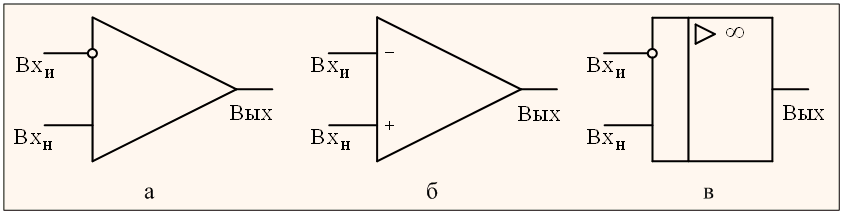
\includegraphics[width=0.7\textwidth]{8_oa_graphic.png}
\caption{УГО операционного усилителя}
\label{fig:8_oa_graphic}
\end{figure}

\subsection*{Основные параметры}

\begin{enumerate}
\item Коэффициент усиления напряжения без обратной связи $K_{u}$, показывающий, во сколько раз напряжение на выходе превышает напряжение сигнала, поданного на дифференциальный вход. Типовое значение $K_{u} = 10^{5} \div 10^{6}$;
\item Коэффициент ослабления синфазного сигнала $K_\text{осл.сф}$, показывающий, во сколько раз дифференциальный сигнал сильнее синфазного. Донный параметр определяется свойствами входного дифференциального каскада и составляет $80 \div 100$ дБ;
\item Напряжение смещения нуля $U_\text{см}$, представляющее собой постоянное напряжение определенной полярности, которое необходимо подать на вход при отсутствии входного сигнала для того, чтобы напряжение на выходе стало равным нулю. Наличие отклонения выходного напряжения от нуля обусловлено, хотя и малым, но неизбежным дисбалансом плеч дифференциального каскада. Практически $U_\text{см} = 5 \div 20$ мВ;
\item Температурный дрейф напряжения смещения $TKU_\text{см} = \dfrac{\Delta U_\text{см}}{\Delta T}$, характеризует изменение напряжения $U_\text{см}$ при изменении температуры и составляет $1 \div 30 \dfrac{\text{мкВ}}{\text{\textcelsius}}$;
\item Входное сопротивление для дифференциального сигнала $R_\text{вх. диф}$. Измеряется со стороны любого входа в то время, когда другой вход соединен с общим выводом. Величина $R_\text{вх. диф}$ лежит в пределах сотен кОм --- единиц МОм;
\item Входное сопротивление для синфазного сигнала $R_\text{вх. сф}$. Измеряется между соединенными вместе входами операционного усилителя и корпусом. Данное сопротивление на несколько порядков больше чем сопротивление для дифференциального сигнала;
\item Выходное сопротивление $R_\text{вых}$. Величина выходного сопротивления для операционного усилителя составляет десятки --- сотни Ом.
\end{enumerate}

\subsection*{Виды ОУ}

\begin{enumerate}
\item Индустриальный стандарт. Так называют широко применяемые, очень дешевые ОУ общего применения со средними характеристиками. Пример ОУ: с биполярным входом --- LM324, с полевым входом --- TL084.
\item Прецизионные ОУ имеют очень малые напряжения смещения, применяются в точных измерительных схемах. Обычно ОУ на биполярных транзисторах по этому показателю несколько лучше, чем на полевых. Также от прецизионных ОУ требуется долговременная стабильность параметров. Исключительно малыми смещениями обладают стабилизированные прерыванием ОУ. Примеры: AD707, AD708, с напряжением смещения 30 мкВ, а также новейшие AD8551 с типичным напряжением смещения 1 мкВ.
\item С малым входным током (электрометрические) ОУ. Все ОУ, имеющие полевые транзисторы на входе, обладают малым входным током. Но среди них существуют специальные ОУ с исключительно малым входным током. Чтобы полностью реализовать их преимущества, при проектировании устройств с их использованием необходимо даже учитывать утечку тока по печатной плате. Пример: AD549 с входным током $6 \ast 10^{-14}$ А.
\item Микромощные и программируемые ОУ потребляют малый ток на собственное питание. Такие ОУ не могут быть быстродействующими, так как малый потребляемый ток и высокое быстродействие --- взаимоисключающие требования. Программируемыми называются ОУ, для которых все внутренние токи покоя можно задать с помощью внешнего тока, подаваемого на специальный вывод ОУ.
\item Мощные (сильноточные) ОУ могут отдавать большой ток в нагрузку, то есть допустимое сопротивление нагрузки меньше стандартных 2 кОм, и может составлять до 50 Ом.
\item Низковольтные ОУ работоспособны при напряжении питания 3 В и даже ниже. Как правило, они имеют rail-to-rail выход.
\item Высоковольтные ОУ. Все напряжения для них (питания, синфазное входное, максимальное выходное) значительно больше, чем для ОУ широкого применения.
\item Быстродействующие ОУ имеют высокую скорость нарастания и частоту единичного усиления. Такие ОУ не могут быть микромощными, и как правило выполнены на биполярных транзисторах.
\item Малошумящие ОУ.
\item Звуковые ОУ. Имеют минимально возможный коэффициент гармоник (THD).
\item Для однополярного питания. CMOS ОУ обеспечивают выходное напряжение, практически равное напряжению питания (rail-to-rail, R2R), биполярные ОУ --- примерно на 1.2 В меньше, что существенно при небольших значениях Ucc.
\item Специализированные ОУ. Обычно разработаны для конкретных задач (подключение фотодатчика, магнитной головки, и др.). Могут содержать в себе готовые цепи ООС или отдельные необходимые для этого прецизионные резисторы.
\end{enumerate}


\subsection*{Балансировка ОУ}

Балансировка ОУ представляет собой операцию по компенсации напряжения смещения в ОУ. Балансировка производится с помощью многооборотного потенциометра Rб , начало и конец которого подключены на входы R ОУ, а средний вывод --- на источник питания Un (-Un). Для балансировки входы ОУ заземляются, и с помощью потенциометра Rб устанавливается напряжение Uвых = 0. Балансировка позволяет компенсировать напряжение смещения ОУ в данный момент при действующих дестабилизирующих факторах. При изменении параметров питающих напряжений и внешних факторов, таких как температура и влажность окружающей среды, балансировка нарушается. Поэтому в ряде случаев применяется автоматическая установка нулей ОУ.

\begin{figure}[H]
\centering
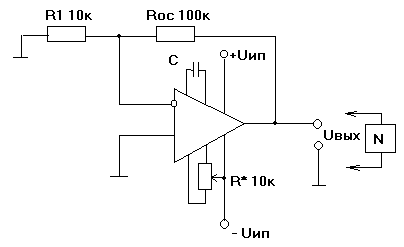
\includegraphics[width=0.5\textwidth]{8_zero_set.png}
\caption{Установка нуля}
\label{fig:8_zero_set}
\end{figure}


% Вопрос 9 --------------------------------------------------------------------
\section{Стабилизаторы напряжения. Классификация. Параметры. Область применения.}

Стабилизатор напряжения --- преобразователь электрической энергии, позволяющий получить на выходе напряжение, находящееся в заданных пределах при значительно больших колебаниях входного напряжения и сопротивления нагрузки.

По типу выходного напряжения стабилизаторы делятся на стабилизаторы постоянного тока и переменного тока. Как правило, тип питания (постоянный либо переменный ток) такой же, как и выходное напряжение, хотя возможны исключения.

Стабилизаторы напряжения подразделяются на однофазные и трехфазные стабилизаторы напряжения.

\subsection*{Классификация стабилизаторов по конструкции}

\begin{itemize}
\item феррорезонансные. Принцип действия основывается на магнитном насыщении сердечников из ферромагнетиков трансформаторов. Этот тип стабилизаторов напряжения был разработан достаточно давно, в начале 60-х годов прошлого века и был призван защитить сложную бытовую технику. Но в настоящее время от их производства отказались почти все производители, из-за очень узкого рабочего диапазона напряжений и невозможности работы прибора без нагрузки.
\item электромеханические. В стабилизаторах этого типа корректировка напряжения производится автоматически, а точность поддержания напряжения достаточно высока (в пределах 3\%).
\item электронные. Этот тип стабилизаторов работает по принципу автоматического переключения трансформаторных секций при помощи силовых ключей (реле, тиристоров и т.д.). Электронные стабилизаторы ступенчатого регулирования обеспечивают выходное напряжение в более широких пределах, чем электромеханические. А также обладают высоким быстродействием и не изменяют форму входного напряжения.
\end{itemize}

\subsection*{Основные параметры стабилизатора}

\begin{itemize}
\item Диапазон входных напряжений(Диапазон напряжений в пределах которого стабилизатор может поддерживать выходное напряжение с заданной точностью)
\item Диапазон  выходных напряжений (Диапазон возможных значений)
\item Точность поддержания выходного напряжения в \%
\item Мощность стабилизатора. Обычно указывается в кВа, это полная мощность.
\end{itemize}

\subsection*{Выбор стабилизатора}

\begin{enumerate}
\item Для выбора стабилизатора необходимо посчитать сумму полных мощностей потребителей, если на потребителе указан $\cos\varphi$ (коэфф. активном мощности в полной), то его учитываем.
\item Определить диапазон изменений напряжений в сети. Произвести изменения максимальных и минимальных напряжений.
\item Выяснить диапазон рабочих напряжений потребителей
\end{enumerate}


% Вопрос 10 ------------------------------------
\section{Логические операции. Схемная реализация.}

Логическая операция --- операция над выражениями булевского типа, соответствующая некоторой операции над высказываниями в алгебре логики. Как и высказывания, логические выражения могут принимать одно из двух истинностных значений --- «истинно» или «ложно». Логические операции служат для получения сложных логических выражений из более простых. В свою очередь, логические выражения обычно используются как условия для управления последовательностью выполнения программы.
Обычно выделяют следующие базовые операции:

\begin{itemize}
\item НЕ (отрицание)
\item И (конъюнкция)
\item ИЛИ (дизъюнкция)
\item XOR (исключающее ИЛИ)
\end{itemize}

Для каждой из операции можно построить простую таблицу истинности.

\begin{figure}[H]
\centering
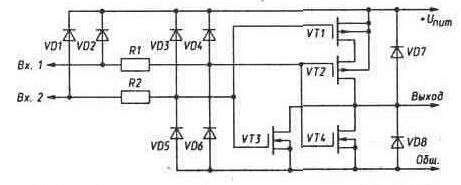
\includegraphics[width=0.7\textwidth]{10_or_not.png}
\caption{Схемная реализация ИЛИ-НЕ}
\label{fig:10_or_not}
\end{figure}

Для всех микросхем существует УГО.


% Вопрос 11 ---------------------------------------------------------------------------------------------------------------
\section{Цифровые устройства. Классификация. Комбинационные ЦУ. Дешифраторы, шифраторы, мультиплексоры, демультиплексоры.}

\subsection*{Виды цифровых устройств}

\begin{enumerate}
\item Логические элементы
\item Триггеры
\item Счётчики
\item Регистры
\item Буферные преобразователи
\item Модули памяти
\item Шифраторы
\item Дешифраторы
\item Цифровой компаратор
\item Мультиплексоры
\item Демультиплексоры
\item Полусумматоры
\item Сумматоры
\item АЛУ
\item Микроконтроллеры
\item (Микро)процессоры
\item Однокристальные микрокомпьютеры
\item ПЛИС --- программируемые логические интегральные схемы
\end{enumerate}

\subsection*{Классификация цифровых устройств}

\begin{itemize}
\item В зависимости от способа ввода и вывода информации:
	\begin{itemize}
	\item Последовательные --- в котором входные сигналы поступают на вход, а выходные сигналы снимаются с выхода последовательно, разряд за разрядом;
	\item Параллельные --- входные сигналы подаются на вход, а выходные снимаются с выхода одновременно;
	\item Последовательно-параллельные --- входные и выходные сигналы представлены в разных формах: либо на вход сигналы поступают последовательно сигнал за сигналом, а с выхода они снимаются одновременно, и наоборот.
	\end{itemize}
\item По принципу действия:
	\begin{itemize}
	\item КЦУ (комбинационные цифр.устр-ва) --- выходные сигналы которых определяются только действующими в данный момент входными сигналами и не зависят от внутреннего состояния устройства.
	\item Последовательностными --- выходные сигналы которых зависят не только от входных сигналов, но и от внутреннего состояния устройства. Этот тип называют цифровыми автоматами.
	\end{itemize}
\end{itemize}

\subsection*{Виды комбинационных ЦУ}
\begin{itemize}
\item дешифраторы
\item шифраторы
\item мультиплексоры
\item демультиплексоры
\item комбинационные сумматоры
\item АЛУ
\end{itemize}


\subsection*{Дешифратор}

Дешифратором называется комбинационная цифровая схема с несколькими входами и выходами, преобразующая код, подаваемый на входы, в сигнал на одном из выходов. Если дешифратор, имеющий n входов, имеет $2^{n}$ выходов, то такой дешифратор называется полным. Если количество выходов меньше, то дешифратор называется неполным.
\begin{figure}[H]
\centering
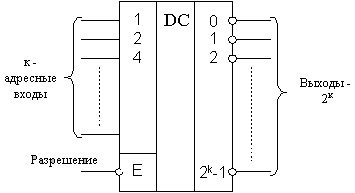
\includegraphics[width=0.5\textwidth]{11_dc.png}
\caption{УГО дешифратора}
\label{fig:11_dc}
\end{figure}

\subsection*{Шифратор}

Шифратором называется устройство, предназначенное для преобразования чисел из десятичной системы в двоичную. Нетрудно видеть, что в шифраторе сигнал, подаваемый на вход X0, не используется. Основное применение шифраторов --- это введение первичной информации с клавиатуры (преобразование десятичного в ДВОИЧНЫЙ), например, ИС К555ИВЗ.
\begin{figure}[H]
\centering
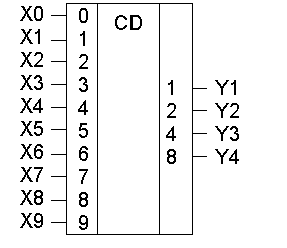
\includegraphics[width=0.4\textwidth]{11_cd.png}
\caption{УГО шифратора}
\label{fig:11_cd}
\end{figure}

\subsection*{Мультиплексор}

Мультиплексором называется комбинационное цифровое устройство, предназначенное для управляемой передачи информации с нескольких источников в один выходной канал. Мультиплексор можно реализовать, используя логические элементы "И" и дешифратор. Мультиплексор имеет один выход, информационные входы и адресные или управляющие входы. В зависимости от кода, подаваемого на адресные шины Х0, Х1 один из информационных входов подключается к выходному каналу.
\begin{figure}[H]
\centering
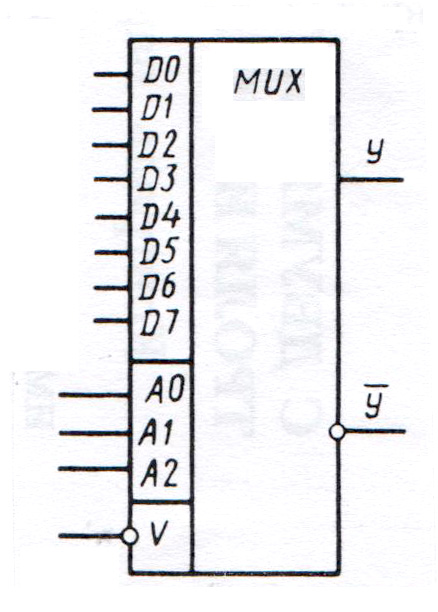
\includegraphics[width=0.25\textwidth]{11_ms.jpg}
\caption{УГО мультиплексора}
\label{fig:11_ms}
\end{figure}

\subsection*{Демультиплексор}

Демультиплексором называется комбинационное логическое устройство, предназначенное для управляемой передачи данных от одного источника информации в несколько выходных каналов. Демультиплексор имеет один информационный вход, n адресных шин и $2^{n}$-выходов.
\begin{figure}[H]
\centering
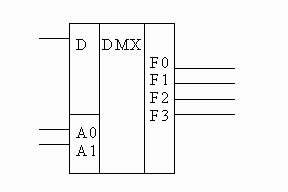
\includegraphics[width=0.45\textwidth]{11_dmx.png}
\caption{УГО демультиплексора}
\label{fig:11_dmx}
\end{figure}


% Вопрос 12 ---------------------------------------------------------------------------------------------------------------
\section{Комбинационные сумматоры.}

Комбинационный сумматор --- это цифровое устройство, пред-назначенное для арифметического сложения чисел, представленных в виде двоичных кодов.

Обычно сумматор представляет собой комбинацию одноразрядных сумматоров. При сложении двух чисел в каждом разряде производится сложение трех цифр: цифры первого слагаемого Ai, цифры второго слагаемого Bi; и цифры переноса из младшего разряда Рi;. В результате суммирования на выходных шинах получается сумма S; и перенос в старший разряд Pj+i.

\begin{figure}[H]
\centering
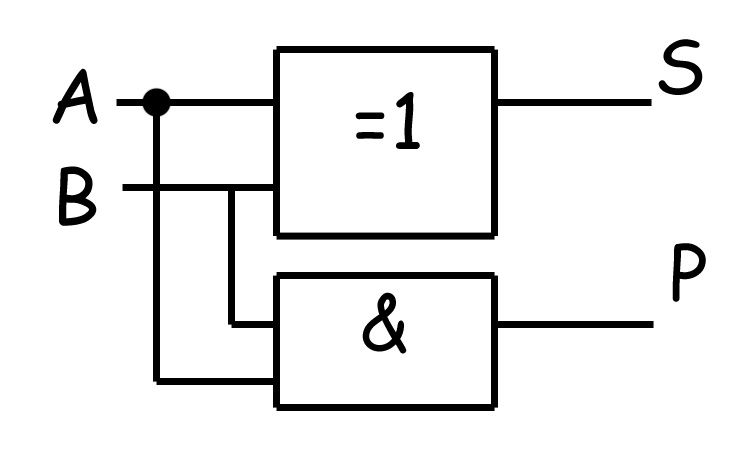
\includegraphics[width=0.3\textwidth]{12_additor.jpg}
\caption{Структура простейшего сумматора}
\label{fig:12_additor}
\end{figure}

\begin{figure}[H]
\centering
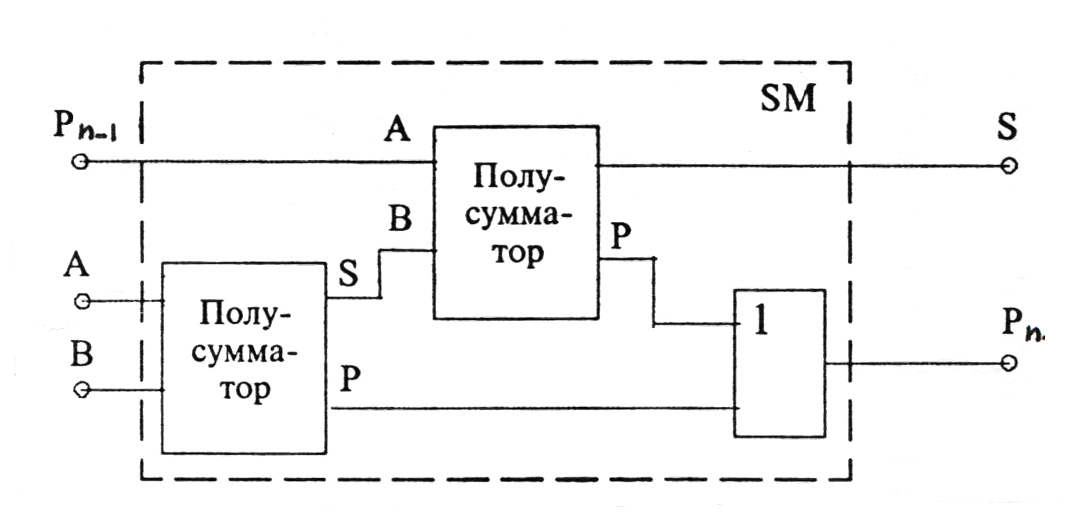
\includegraphics[width=0.7\textwidth]{12_cs.jpg}
\caption{Структура комбинационного сумматора}
\label{fig:12_cs}
\end{figure}


% Вопрос 13 ---------------------------------------------------------------------------------------------------------------
\section{Триггера. Классификация. Область применения.}

Триггером называется цифровое устройство, которое может находиться в одном из двух устойчивых состояний и переходит из одного состояния в другое под действием входных сигналов. Триггеры можно классифицировать по способу приема информации, принципу построения, функциональным возможностям. По способу приема информации триггеры подразделяются на асинхронные и синхронные. Асинхронный триггер изменяет свое состояние в момент прихода сигнала на его информационные входы. Синхронные триггеры изменяют свое состояние под воздействием входных сигналов только в момент прихода активного сигнала на его синхронизирующий вход С.

По виду активного сигнала, действующего на информационных входах, триггеры подразделяются на статические и динамические. Первые переключаются потенциалом (уровнем напряжения), а вторые --- перепадом (передним или задним фронтом импульса). Входные информационные сигналы могут быть прямыми и инверсными.

\subsection*{Асинхронный RS-триггер}

RS-триггер --- триггер, который сохраняет своё предыдущее состояние при нулевых входах и меняет своё выходное состояние при подаче на один из его входов единицы.

Таблица истинности асинхронного RS-триггера.

\begin{tabular}{|c|c|c|}
\hline	S	& R	& Q			\\
\hline	0	& 0	& Q(n-1)	\\
\hline	0	& 1	& 0			\\
\hline	1	& 0	& 1			\\
\hline	1	& 1	& X			\\
\hline
\end{tabular}

\subsection*{Синхронный RS-триггер}

Синхронный RS-триггер очень похож на асинхронный, с тем лишь различием, что имеется вход синхронизации, при 1 на котором и происходит работа.

Таблица истинности синхронного RS-триггера.

\begin{tabular}{|c|c|c|c|c|}
\hline	C	& S	& R	& Q(t)	& Q(t+1)	\\
\hline	0	& X	& X	& 0		& 0			\\
\hline	0	& X	& X	& 1		& 1			\\
\hline	1	& 0	& 0	& 0		& 0			\\
\hline	1	& 0	& 0	& 1		& 1			\\
\hline	1	& 0	& 1	& 0		& 0			\\
\hline	1	& 0	& 1	& 1		& 0			\\
\hline	1	& 1	& 0	& 0		& 1			\\
\hline	1	& 1	& 0	& 1		& 1			\\
\hline	1	& 1	& 1	& 0		& не опред.	\\
\hline	1	& 1	& 1	& 1		& не опред.	\\
\hline
\end{tabular}

\subsection*{D-триггер}

D-триггер --- запоминает состояние входа и выдаёт его на выход. D-триггеры имеют, как минимум, два входа: информационный D и синхронизации С. После прихода активного фронта импульса синхронизации на вход С D-триггер открывается. Сохранение информации в D-триггерах происходит после спада импульса синхронизации С. Так как информация на выходе остаётся неизменной до прихода очередного импульса синхронизации, D-триггер называют также триггером с запоминанием информации или триггером-защёлкой. Рассуждая чисто теоретически, парафазный (двухфазный) D-триггер можно образовать из любых RS- или JK-триггеров, если на их входы одновременно подавать взаимно инверсные сигналы.

D-триггер в основном используется для реализации защёлки. Так, например, для снятия 32 бит информации с параллельной шины, берут 32 D-триггера и объединяют их входы синхронизации для управления записью информации в защёлку, а 32 D входа подсоединяют к шине.

В одноступенчатых D-триггерах во время прозрачности все изменения информации на входе D передаются на выход Q. Там, где это нежелательно, нужно применять двухступенчатые (двухтактные, Master-Slave, MS) D-триггеры.

Таблица истинности синхронного D-триггера.

\begin{tabular}{|c|c|c|}
\hline	D	& Q(t)	& Q(t+1)	\\
\hline	0	& 0		& 0			\\
\hline	0	& 1		& 0			\\
\hline	1	& 0		& 1			\\
\hline	1	& 1		& 1			\\
\hline
\end{tabular}

\subsection*{T-триггер}

Синхронный Т-триггер, при единице на входе Т, по каждому такту на входе С изменяет своё логическое состояние на противоположное, и не изменяет выходное состояние при нуле на входе T. Т-триггер можно построить на JK-триггере, на двухступенчатом (Master-Slave, MS) D-триггере и на двух одноступенчатых D-триггерах и инверторе.

Как можно видеть в таблице истинности JK-триггера, он переходит в инверсное состояние каждый раз при одновременной подаче на входы J и K логической 1. Это свойство позволяет создать на базе JK-триггера Т-триггер, объединяя входы J и К.

В двухступенчатом (Master-Slave, MS) D-триггере инверсный выход Q соединяется со входом D, а на вход С подаются счётные импульсы. В результате триггер при каждом счётном импульсе запоминает значение Q, то есть будет переключаться в противоположное состояние.

Т-триггер часто применяют для понижения частоты в 2 раза, при этом на Т вход подают единицу, а на С --- сигнал с частотой, которая будет поделена на 2.

Таблица истинности синхронного T-триггера.

\begin{tabular}{|c|c|c|}
\hline	T	& Q(t)	& Q(t+1)	\\
\hline	0	& 0		& 0			\\
\hline	0	& 1		& 1			\\
\hline	1	& 0		& 1			\\
\hline	1	& 1		& 0			\\
\hline
\end{tabular}

\subsection*{JK-триггер}

JK-триггер работает так же как RS-триггер, с одним лишь исключением: при подаче логической единицы на оба входа J и K состояние выхода триггера изменяется на противоположное. Вход J (от англ. Jump --- прыжок) аналогичен входу S у RS-триггера. Вход K (от англ. Kill --- убить) аналогичен входу R у RS-триггера. При подаче единицы на вход J и нуля на вход K выходное состояние триггера становится равным логической единице. А при подаче единицы на вход K и нуля на вход J выходное состояние триггера становится равным логическому нулю. JK-триггер в отличие от RS-триггера не имеет запрещённых состояний на основных входах, однако это никак не помогает при нарушении правил разработки логических схем. На практике применяются только синхронные JK-триггеры, то есть состояния основных входов J и K учитываются только в момент тактирования, например по положительному фронту импульса на входе синхронизации.

На базе JK-триггера возможно построить D-триггер или Т-триггер. Как можно видеть в таблице истинности JK-триггера, он переходит в инверсное состояние каждый раз при одновременной подаче на входы J и K логической 1. Это свойство позволяет создать на базе JK-триггера Т-триггер, объединив входы J и К.

Таблица истинности синхронного JK-триггера.

\begin{tabular}{|c|c|c|c|}
\hline	J	& K	& Q(t)	& Q(t+1)	\\
\hline	0	& 0	& 0		& 0			\\
\hline	0	& 0	& 1		& 1			\\
\hline	0	& 1	& 0		& 0			\\
\hline	0	& 1	& 1		& 0			\\
\hline	1	& 0	& 0		& 1			\\
\hline	1	& 0	& 1		& 1			\\
\hline	1	& 1	& 0		& 1			\\
\hline	1	& 1	& 1		& 0			\\
\hline
\end{tabular}


% Вопрос 14 ---------------------------------------------------------------------------------------------------------------
\section{Регистры и счетчики. Классификация. Схемы. Область применения.}

Регистр --- последовательное или параллельное логическое устройство, используемое для хранения n-разрядных двоичных чисел и выполнения преобразований над ними.

Регистр представляет собой упорядоченную последовательность триггеров, обычно D, число которых соответствует числу разрядов в слове. С каждым регистром обычно связано комбинационное цифровое устройство, с помощью которого обеспечивается выполнение некоторых операций над словами.

Фактически любое цифровое устройство можно представить в виде совокупности регистров, соединённых друг с другом при помощи комбинационных цифровых устройств.

Основой построения регистров являются D-триггеры, RS-триггеры.

\begin{figure}[H]
\centering
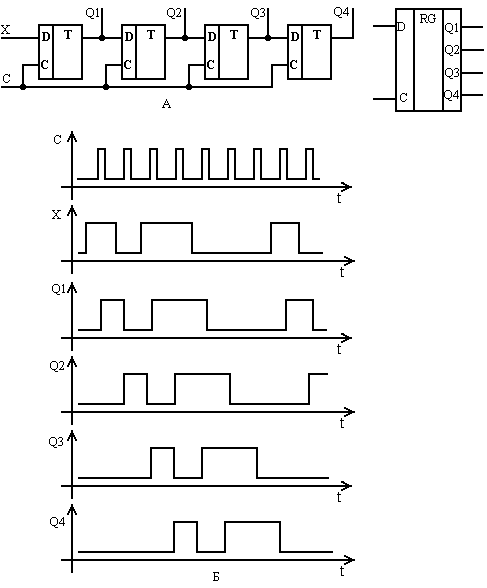
\includegraphics[width=0.6\textwidth]{14_register.png}
\caption{Регистр: схема реализации, УГО, схема сигналов}
\label{fig:14_register}
\end{figure}

\subsection*{Классификация регистров}

\begin{itemize}
\item накопительные;
\item сдвигающие. Которые в свою очередь делятся на:
	\begin{itemize}
	\item по способу ввода-вывода информации:
		\begin{itemize}
		\item параллельные
			\par запись и считывание информации происходит одновременно на все входы и со всех выходов
		\item последовательные
			\par запись и считывание информации происходит в первый триггер, а та информация, которая была в этом триггере, перезаписывается в следующий --- то же самое происходит и с остальными триггерами
		\item комбинированные
		\end{itemize}
	\item по направлению передачи информации:
		\begin{itemize}
			\item однонаправленные
			\item реверсивные
		\end{itemize}
	\item по основанию системы счисления:
		\begin{itemize}
			\item двоичные
			\item троичные
			\item десятичные
		\end{itemize}
	\end{itemize}
\end{itemize}

Счётчик числа импульсов --- устройство, на выходах которого получается двоичный (двоично-десятичный) код, определяемый числом поступивших импульсов. Счётчики могут строиться на двухступенчатых D-триггерах, T-триггерах и JK-триггерах.

Основной параметр счётчика --- модуль счёта --- максимальное число единичных сигналов, которое может быть сосчитано счётчиком. Счётчики обозначают через СТ (от англ. counter).

\subsection*{Классификация счетчиков}

\begin{itemize}
\item по числу устойчивых состояний триггеров
	\begin{itemize}
	\item на двоичных триггерах
	\item на троичных триггерах
	\item на n-ичных триггерах
	\end{itemize}
\item по модулю счёта:
	\begin{itemize}
	\item двоично-десятичные (декада)
	\item двоичные
	\item с произвольным постоянным модулем счёта
	\item с переменным модулем счёта
	\end{itemize}
\item по направлению счёта:
	\begin{itemize}
	\item суммирующие
	\item вычитающие
	\item реверсивные
	\end{itemize}
\item по способу формирования внутренних связей:
	\begin{itemize}
	\item с последовательным переносом
	\item с ускоренным переносом
		\begin{itemize}
		\item с параллельным ускоренным переносом
		\item со сквозным ускоренным переносом
		\end{itemize}
	\item с комбинированным переносом
	\item кольцевые
	\end{itemize}
\item по способу переключения триггера:
	\begin{itemize}
	\item синхронные
	\item асинхронные
	\end{itemize}
\item Счётчик Джонсона
	\par Счетчиком Джонсона называют кольцевой регистр, который строится на основе замкнутого регистра сдвига с одной перекрестной инверсной связью. Счетчик имеет коэффициент пересчета, вдвое больший числа составляющих его триггеров.
\end{itemize}


% Вопрос 15 ---------------------------------------------------------------------------------------------------------------
\section{Цифро-аналоговые преобразователи. Назначение. Принцип работы. Матрица R-2R. Область применения.}

Цифро-аналоговый преобразователь (ЦАП) --- устройство для преобразования цифрового (обычно двоичного) кода в аналоговый сигнал (ток, напряжение или заряд). Цифро-аналоговые преобразователи являются интерфейсом между дискретным цифровым миром и аналоговыми сигналами.

Наиболее общие типы электронных ЦАП:

\begin{itemize}
\item Широтно-импульсный модулятор --- простейший тип ЦАП. Стабильный источник тока или напряжения периодически включается на время, пропорциональное преобразуемому цифровому коду, далее полученная импульсная последовательность фильтруется аналоговым фильтром нижних частот. Такой способ часто используется для управления скоростью электромоторов, а также становится популярным в Hi-Fi-аудиотехнике;

\item ЦАП передискретизации, такие как дельта-сигма-ЦАП, основаны на изменяемой плотности импульсов. Передискретизация позволяет использовать ЦАП с меньшей разрядностью для достижения большей разрядности итогового преобразования; часто дельта-сигма ЦАП строится на основе простейшего однобитного ЦАП, который является практически линейным. На ЦАП малой разрядности поступает импульсный сигнал с модулированной плотностью импульсов (c постоянной длительностью импульса, но с изменяемой скважностью), создаваемый с использованием отрицательной обратной связи. Отрицательная обратная связь выступает в роли фильтра верхних частот для шума квантования.

\item Большинство ЦАП большой разрядности (более 16 бит) построены на этом принципе вследствие его высокой линейности и низкой стоимости. Быстродействие дельта-сигма ЦАП достигает сотни тысяч отсчетов в секунду, разрядность --- до 24 бит. Для генерации сигнала с модулированной плотностью импульсов может быть использован простой дельта-сигма модулятор первого порядка или более высокого порядка как MASH (англ. Multi stage noise SHaping). С увеличением частоты передискретизации смягчаются требования, предъявляемые к выходному фильтру низких частот и улучшается подавление шума квантования;

\item ЦАП взвешивающего типа, в котором каждому биту преобразуемого двоичного кода соответствует резистор или источник тока, подключенный на общую точку суммирования. Сила тока источника (проводимость резистора) пропорциональна весу бита, которому он соответствует. Таким образом, все ненулевые биты кода суммируются с весом. Взвешивающий метод один из самых быстрых, но ему свойственна низкая точность из-за необходимости наличия набора множества различных прецизионных источников или резисторов и непостоянного импеданса. По этой причине взвешивающие ЦАП имеют разрядность не более восьми бит;

\item ЦАП лестничного типа (цепная R-2R-схема). В R-2R-ЦАП значения создаются в специальной схеме, состоящей из резисторов с сопротивлениями R и 2R, называемой матрицей постоянного импеданса, которая имеет два вида включения: прямое --- матрица токов и инверсное --- матрица напряжений. Применение одинаковых резисторов позволяет существенно улучшить точность по сравнению с обычным взвешивающим ЦАП, так как сравнительно просто изготовить набор прецизионных элементов с одинаковыми параметрами. ЦАП типа R-2R позволяют отодвинуть ограничения по разрядности. С лазерной подгонкой резисторов на одной подложке достигается точность 20-22 бита. Основное время на преобразование тратится в операционном усилителе, поэтому он должен иметь максимальное быстродействие. Быстродействие ЦАП единицы микросекунд и ниже (то есть наносекунды);
\end{itemize}

ЦАП находятся в начале аналогового тракта любой системы, поэтому параметры ЦАП во многом определяют параметры всей системы в целом. Далее перечислены наиболее важные характеристики ЦАП.

\begin{itemize}
\item Разрядность --- количество различных уровней выходного сигнала, которые ЦАП может воспроизвести. Обычно задается в битах; количество бит есть логарифм по основанию 2 от количества уровней. Например, однобитный ЦАП способен воспроизвести два ($2^1$) уровня, а восьмибитный --- 256 ($2^8$) уровней. Разрядность тесно связана с эффективной разрядностью (англ. ENOB, Effective Number of Bits), которая показывает реальное разрешение, достижимое на данном ЦАП.

\item Максимальная частота дискретизации --- максимальная частота, на которой ЦАП может работать, выдавая на выходе корректный результат. В соответствии с теоремой Найквиста --- Шеннона (известной также как теорема Котельникова), для корректного воспроизведения аналогового сигнала из цифровой формы необходимо, чтобы частота дискретизации была не менее, чем удвоенная максимальная частота в спектре сигнала. Например, для воспроизведения всего слышимого человеком звукового диапазона частот, спектр которого простирается до 20 кГц, необходимо, чтобы звуковой сигнал был дискретизован с частотой не менее 40 кГц. Стандарт Audio CD устанавливает частоту дискретизации звукового сигнала 44,1 кГц; для воспроизведения данного сигнала понадобится ЦАП, способный работать на этой частоте. В дешевых компьютерных звуковых картах частота дискретизации составляет 48 кГц. Сигналы, дискретизованные на других частотах, подвергаются передискретизации до 48 кГц, что частично ухудшает качество сигнала.

\item Монотонность --- свойство ЦАП увеличивать аналоговый выходной сигнал при увеличении входного кода.

\item THD+N (суммарные гармонические искажения + шум) --- мера искажений и шума вносимых в сигнал ЦАПом. Выражается в процентах мощности гармоник и шума в выходном сигнале. Важный параметр при малосигнальных применениях ЦАП.

\item Динамический диапазон --- соотношение наибольшего и наименьшего сигналов, которые может воспроизвести ЦАП, выражается в децибелах. Данный параметр связан с разрядностью и шумовым порогом.

\item Статические характеристики:
	\begin{itemize}
	\item DNL (дифференциальная нелинейность) --- характеризует, насколько приращение аналогового сигнала, полученное при увеличении кода на 1 младший значащий разряд (МЗР), отличается от правильного значения;
	\item INL (интегральная нелинейность) --- характеризует, насколько передаточная характеристика ЦАП отличается от идеальной. Идеальная характеристика строго линейна; INL показывает, насколько напряжение на выходе ЦАП при заданном коде отстоит от линейной характеристики; выражается в МЗР;
	\item усиление;
	\item смещение.
	\end{itemize}

\item Частотные характеристики:
	\begin{itemize}
	\item SNDR (отношение сигнал/шум+искажения) --- характеризует в децибелах отношение мощности выходного сигнала к суммарной мощности шума и гармонических искажений;
	\item HDi (коэффициент i-й гармоники) --- характеризует отношение i-й гармоники к основной гармонике;
	\item THD (коэффициент гармонических искажений) --- отношение суммарной мощности всех гармоник (кроме первой) к мощности первой гармоники.
	\end{itemize}
\end{itemize}

\begin{figure}[H]
\centering
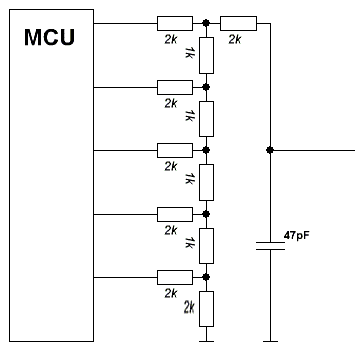
\includegraphics[width=0.5\textwidth]{15_R2R.png}
\caption{Схема R2R-матрицы}
\label{fig:15_R2R}
\end{figure}


% Вопрос 16 ---------------------------------------------------------------------------------------------------------------
\section{Аналого-цифровые преобразователи. Классификация. Область применения. Параллельные АЦП. АЦП поразрядного взвешивания.}

Аналого-цифровой преобразователь (АЦП, англ. Analog-to-digital converter, ADC) --- устройство, преобразующее входной аналоговый сигнал в дискретный код (цифровой сигнал). Обратное преобразование осуществляется при помощи ЦАП (цифро-аналогового преобразователя, DAC).

Как правило, АЦП --- электронное устройство, преобразующее напряжение в двоичный цифровой код. Тем не менее, некоторые неэлектронные устройства с цифровым выходом, следует также относить к АЦП, например, некоторые типы преобразователей угол-код. Простейшим одноразрядным двоичным АЦП является компаратор.

\begin{figure}[H]
\centering
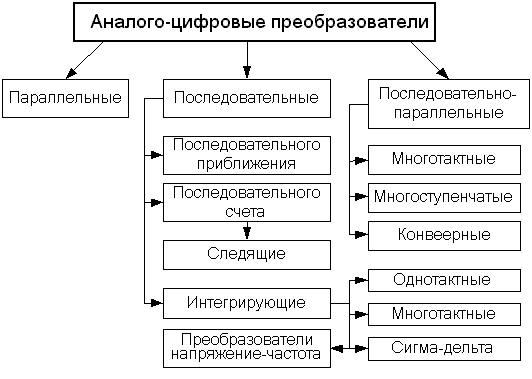
\includegraphics[width=0.7\textwidth]{16_ADC_scheme.png}
\caption{Классификация АЦП}
\label{fig:16_ADC_scheme}
\end{figure}

\subsection*{АЦП параллельного типа}
АЦП параллельного типа осуществляют квантование сигнала одновременно с помощью набора компараторов, включенных параллельно источнику входного сигнала. Ниже показана реализация параллельного метода АЦ-преобразования для 3-разрядного числа.

\begin{figure}[H]
\centering
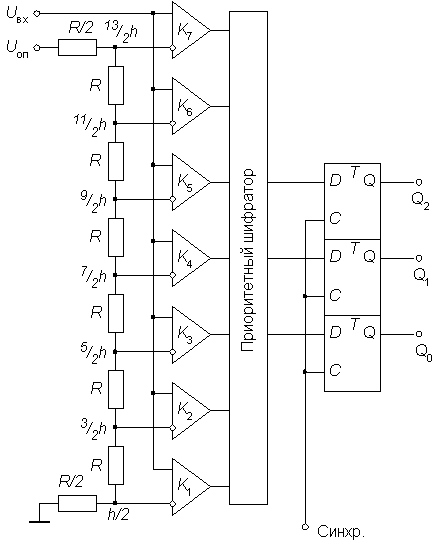
\includegraphics[width=0.6\textwidth]{16_parallel_ADC.png}
\caption{Устройство параллельного АЦП}
\label{fig:16_parallel_ADC}
\end{figure}

С помощью трех двоичных разрядов можно представить восемь различных чисел, включая нуль. Необходимо, следовательно, семь компараторов. Семь соответствующих эквидистантных опорных напряжений образуются с помощью резистивного делителя.

Параллельный АЦП является не только самым простым преобразователем с точки зрения операционной, но также и самым быстрым из всех типов АЦП, причём скорость работы ограничивается лишь задержкой на прохождение сигнала на логическом элементе и компараторе. К сожалению, в состав параллельных АЦП входит большое количество компонентов, причём размер схемы тем больше, чем выше разрядность АЦП. Для трёхразрядного АЦП требуются семь компараторов. В четырёхразрядной модели используется уже пятнадцать компараторов. По мере увеличения разрядности на одну единицу количество требуемых компараторов удваивается. Принимая в расчёт то, что восемь разрядов обычно считаются минимальным числом для обеспечения достаточной точности АЦП (то есть в случае параллельного АЦП необходимо 255 компараторов!), выявляется основная слабость технологии параллельных АЦП.

Другим, обычно не учитываемым, достоинством параллельных АЦП является возможность работы в нелинейном режиме. В случае использования в цепи делителя напряжения резисторов с равным номиналом каждый следующий импульс двоичного кода будет представлять одно и то же приращение аналогового сигнала, что будет обеспечивать пропорциональный выход. Однако в особых случаях в цепи делителя могут применяться резисторы с различными номиналами. Так образом реализуется нелинейный отклик на аналоговый входной сигнал. Никакой иной тип АЦП не позволяет обеспечить подобное преобразование сигнала путём простого изменением номиналов нескольких компонентов.

\subsection*{АЦП с поразрядным уравновешиванием}

АЦП с поразрядным уравновешиванием, является наиболее распространенным вариантом последовательных АЦП.

В основе работы этого класса преобразователей лежит принцип дихотомии, т.е последовательного сравнения измеряемой величины с 1/2, 1/4, 1/8 и т.д. от возможного максимального значения ее. Это позволяет для N-разрядного АЦП последовательного приближения выполнить весь процесс преобразования за N последовательных шагов (итераций) вместо $2^{N-1}$ при использовании последовательного счета и получить существенный выигрыш в быстродействии. Так, уже при N=10 этот выигрыш достигает 100 раз и позволяет получить с помощью таких АЦП до $10^5$...$10^6$ преобразований в секунду. В то же время статическая погрешность этого типа преобразователей, определяемая в основном используемым в нем ЦАП, может быть очень малой, что позволяет реализовать разрешающую способность до 18 двоичных разрядов при частоте выборок до 200 кГц (например, DSP101 фирмы Burr-Brown).

\begin{figure}[H]
\centering
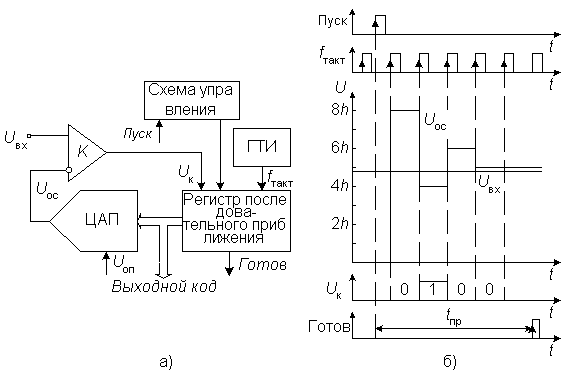
\includegraphics[width=0.8\textwidth]{16_ADC_serial_approx.png}
\caption{а) Устройство АЦП поразрядного взвешивания; б) Временная диаграмма}
\label{fig:16_ADC_serial_approx}
\end{figure}


% Вопрос 17 ---------------------------------------------------------------------------------------------------------------
\section{Интегрирующие АЦП. АЦП двойного интегрирования.}

\subsection*{Общие особенности}

АЦП данного типа осуществляют преобразование в два этапа.

\begin{enumerate}
\item На первом этапе входной аналоговый сигнал интегрируется и это проинтегрированное значение преобразуется в импульсную последовательность. Частота следования импульсов в этой последовательности или их длительность бывает промодулирована проинтегрированным значением входного сигнала.
\item На втором этапе эта последовательность импульсов преобразуется в цифровой код --- измеряется ее частота или длительность импульсов.
\end{enumerate}

\subsection*{Общие достоинства}

\begin{enumerate}
\item АЦП данного типа нечувствительны к импульсным помехам.
\item АЦП данного типа нечувствительны к периодическим помехам если их период в целое число раз меньше периода интегрирования.
\item В результате, АЦП данного типа являются наиболее точными --- типичная точность --- 4...6 десятичных знаков, что соответствует 14...20 двоичным разрядам.
\item При работе АЦП данного типа в составе микропроцессорной системы возможна программная реализация части измерительной процедуры, а именно второго этапа --- измерения временных характеристик последовательности импульсов, что упрощает преобразователь.
\end{enumerate}

\subsection*{Общие недостатки}

Преобразователи данного типа являются наименее быстродействующими из всех --- типичное время преобразования --- 1 - 1000 мс.

\subsection*{Программная реализация части преобразовательной процедуры}

Как уже отмечалось, при работе АЦП данного типа в составе микропроцессорной системы возможна программная реализация части измерительной процедуры, а именно второго этапа --- измерения временных характеристик последовательности импульсов. Это измерение возможно как чисто программно при отсчете времени по счетчику команд или циклов, так и с использованием таймеров. В частности, для данных целей очень хорошо подходит устройство PCA, входящее в состав расширенных вариантов микроконтроллеров семейства MCS-51.

\subsection*{Классификация и примеры построения}

АЦП данного типа классифицируются, как правило, по типу преобразователя напряжение --- импульная последовательность. Бывают преобразователи напряжение-частота (ПНЧ) либо --- напряжение-время (ПНВ). Кроме того возможно построение преобразователей с постоянным тактом, циклом, зарядом или напряжением. Рассмотрим два варианта построения интегрирующих АЦП

\subsection*{АЦП с двойным интегрированием}

Это двухтактный преобразователь с заданной длительностью первого такта.

В течении первого такта происходит заряд интегрирующего конденсатора. Напряжение на нем в конце такта пропорционально интегралу входного напряжения.

Во время второго такта преобразования происходит разряд конденсатора заданным током до нулевого напряжения. Длительность этого такта и есть выходной сигнал преобразователя.

Достоинством данного варианта построения интегрирующего АЦП является не зависимость результата преобразователя от емкости интегрирующего конденсатора и пропорциональное изменение длительности второго такта при изменении длительности первого. Это позволяет снизить требования к точности тактовой частоты. В результате именно этот тип преобразователя используется в большинстве цифровых измерительных приборах.

\begin{figure}[H]
\centering
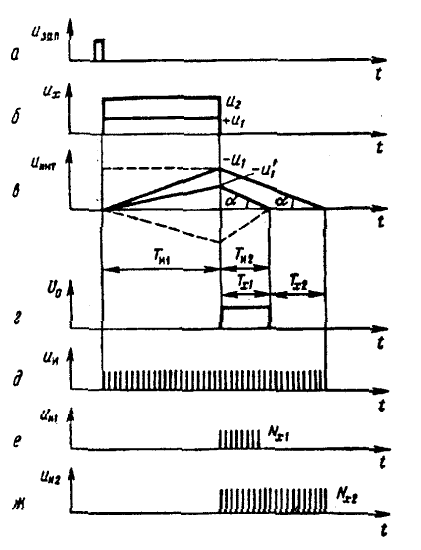
\includegraphics[width=0.5\textwidth]{17_ADC_2INT.png}
\caption{АЦП двойного интегрирования}
\label{fig:17_ADC_2INT}
\end{figure}


% Вопрос 18 ---------------------------------------------------------------------------------------------------------------
\section{Таймеры. Классификация. Область применения.}

Таймером называется устройство, предназначенное для формирования импульсных сигналов с регулируемой длительностью и скважностью. Таймеры делятся на две группы: однотактные и многотактные.

Однотактные таймеры применяются для формирования импульсов длительностью от 1 мкс до минут  и более. Многотактные таймеры включают в себя однотактный таймер и счетчик и предназначены для формирования временных интервалов длительностью в десятки часов.

Наиболее распространенным типом однотактного таймера является ИС К1006ВИ1 (NE555). Функциональная схема таймера приведена на рисунке ниже.

\begin{figure}[H]
\centering
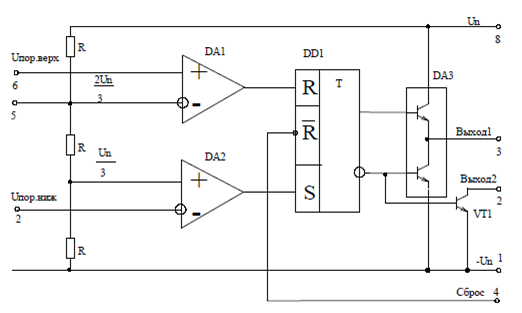
\includegraphics[width=0.6\textwidth]{18_scheme.png}
\caption{Схема таймера}
\label{fig:18_scheme_2INT}
\end{figure}

Таймер состоит из четырех функциональных устройств: двух компараторов DA1 и DA2,  RS-триггера  DD1, усилителя мощности DA3. Внутренний резистивный делитель задает пороговые напряжения, равные, 2Uп/3 для компаратора DA1 и Uп/3 для компаратора DA2. Напряжение питания Uп = 5 - 16,5в, потребляемый ток Iп = 0,7 Uп. Входные токи таймера не превышают 0,5 мкА. Максимальная частота 10 МГц. Таймер имеет второй высокоомный выход к.7.

Таймеры широко используются во многих импульсных устройствах.

На основе таймеров могут быть построены мультивибраторы, одновибраторы, преобразователи напряжения. Таймеры могут входить в состав аппаратуры систем автоматического управления. Особенностью таймеров является высокая стабильность их работы в широком интервале температур.

На рис приведена схема одновибратора, выполненная на таймере К1006ВИ1.

\begin{figure}[H]
\centering
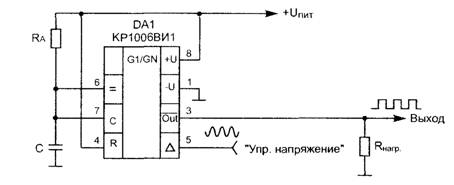
\includegraphics[width=0.5\textwidth]{18_1vibe.jpg}
\caption{Схема одновибратора на К1006ВИ1}
\label{fig:18_1vibe}
\end{figure}

Для работы таймера в режиме одновибратора на объединенные входы к.7 и 6 подключается цепочка RC. При поступлении на вход 2 запускающего импульса амплитудой, меньше Uп/3, триггер DD1 переворачивается, и на выходе 1 формируется прямоугольный импульс. Одновременно запирается транзистор VT1, и конденсатор С начинает заряжаться через резистор R. Напряжение Uс на входах 6,7 возрастает по экспоненте и в момент времени t2 достигает уровня 2Uп/3.

При этом срабатывает компаратор DA1, триггер DD1 возвращается в первоначальное состояние, открывается транзистор VT1, конденсатор С разряжается, и формируется задний фронт импульса на выходе 1. Длительность импульса Ти зависит от постоянной времени RC. Длительность импульса Ти = 1,1 RC.

Схема мультивибратора на базе таймера приведена на рисунке ниже.

\begin{figure}[H]
\centering
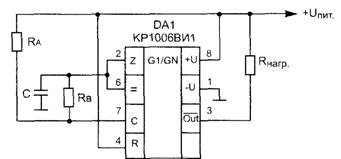
\includegraphics[width=0.5\textwidth]{18_Mvibe.jpg}
\caption{Схема мультивибратора на базе таймера}
\label{fig:18_Mvibe}
\end{figure}

Здесь входы к2 и к6 объединены и подключены на интегрирующую цепочку RC. Напряжение на емкости С UС меняется по экспоненциальному закону между уровнями Uп/3 и 2Uп/3. Период импульсов мультивибратора равен Т = 1,4 RC. Скважность равна 2.

Существует большое количество других схем, построенных на базе таймера К1006ВИ1 (детектор пропущенных импульсов, фазоимпульсный модулятор...).


% Вопрос 19 ---------------------------------------------------------------------------------------------------------------
\section{Источники вторичного напряжения. Структурные схемы. Выпрямители и фильтры.}

Вторичный источник электропитания --- это устройство, предназначенное для обеспечения питания электроприбора электрической энергией, при соответствии требованиям её параметров: напряжения, тока, и т. д. путём преобразования энергии других источников питания. Согласно ГОСТ Р 52907-2008 слово «вторичный» опускается.

\subsection*{Классификация}

\begin{itemize}
\item Обеспечение передачи мощности --- источник питания должен обеспечивать передачу заданной мощности с наименьшими потерями и соблюдением заданных характеристик на выходе без вреда для себя. Обычно мощность источника питания берут с некоторым запасом.
\item Преобразование формы напряжения --- преобразование переменного напряжения в постоянное, и наоборот, а также преобразование частоты, формирование импульсов напряжения и т. д. Чаще всего необходимо преобразование переменного напряжения промышленной частоты в постоянное.
\item Преобразование величины напряжения --- как повышение, так и понижение. Нередко необходим набор из нескольких напряжений различной величины для питания различных цепей.
\item Стабилизация --- напряжение, ток и другие параметры на выходе источника питания должны лежать в определённых пределах, в зависимости от его назначения при влиянии большого количества дестабилизирующих факторов: изменения напряжения на входе, тока нагрузки и т. д. Чаще всего необходима стабилизация напряжения на нагрузке, однако иногда (например, для зарядки аккумуляторов) необходима стабилизация тока.
\item Защита --- напряжение, или ток нагрузки в случае неисправности (например, короткого замыкания) каких-либо цепей может превысить допустимые пределы и вывести электроприбор, или сам источник питания из строя. Также во многих случаях требуется защита от прохождения тока по неправильному пути: например прохождения тока через землю при прикосновении человека или постороннего предмета к токоведущим частям.
\item Гальваническая развязка цепей --- одна из мер защиты от протекания тока по неверному пути.
\item Регулировка --- в процессе эксплуатации может потребоваться изменение каких-либо параметров для обеспечения правильной работы электроприбора.
\item Управление --- может включать регулировку, включение/отключение каких-либо цепей, или источника питания в целом. Может быть как непосредственным (с помощью органов управления на корпусе устройства), так и дистанционным, а также программным (обеспечение включения/выключения, регулировка в заданное время или с наступлением каких-либо событий).
\item Контроль --- отображение параметров на входе и на выходе источника питания, включения/выключения цепей, срабатывания защит. Также может быть непосредственным или дистанционным.
\end{itemize}

\subsection*{Трансформаторные ВИП}

Классическим блоком питания является трансформаторный БП. В общем случае он состоит из понижающего трансформатора или автотрансформатора, у которого первичная обмотка рассчитана на сетевое напряжение. Затем устанавливается выпрямитель, преобразующий переменное напряжение в постоянное (пульсирующее однонаправленное). В большинстве случаев выпрямитель состоит из одного диода (однополупериодный выпрямитель) или четырёх диодов, образующих диодный мост (двухполупериодный выпрямитель). Иногда используются и другие схемы, например, в выпрямителях с удвоением напряжения. После выпрямителя устанавливается фильтр, сглаживающий колебания (пульсации). Обычно он представляет собой просто конденсатор большой ёмкости.

Также в схеме могут быть установлены фильтры высокочастотных помех, всплесков (варисторы), защиты от КЗ, стабилизаторы напряжения и тока.

\begin{figure}[H]
\centering
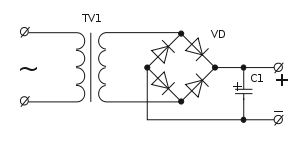
\includegraphics[width=0.8\textwidth]{19_transformer.png}
\caption{Схема простейшего трансформаторного ВИП}
\label{fig:19_transformer}
\end{figure}

\textbf{Структурная схема: трансформатор -> выпрямитель -> сглаживающий фильтр -> стабилизатор}

Достоинства трансформаторных БП:

\begin{itemize}
\item Простота конструкции.
\item Надёжность.
\item Доступность элементной базы.
\item Отсутствие создаваемых радиопомех (в отличие от импульсных, создающих помехи за счет гармонических составляющих).
\end{itemize}

Недостатки трансформаторных БП:

\begin{itemize}
\item Большой вес и габариты, пропорционально мощности.
\item Металлоёмкость.
\item Компромисс между снижением КПД и стабильностью выходного напряжения: для обеспечения стабильного напряжения требуется стабилизатор, вносящий дополнительные потери.
\item Слабая стойкость оборудования с таким БП к броскам напряжения и «отгоранию нуля» (обычно возникает в воздушных сетях сельской местности, приводит к повышению напряжения в розетках с 220 до 380 В). Печально известны в этом плане платы автоматики отопительных котлов (как правило они защищаются варистором, но часто и этого оказывается недостаточно). В то же время техника с импульсными БП (например, современные телевизоры) часто переносит повышения питания до 380 В без разрушения.
\end{itemize}

\subsection*{Импульсные ВИП}

Импульсные блоки питания являются инверторной системой. В импульсных блоках питания переменное входное напряжение сначала выпрямляется. Полученное постоянное напряжение преобразуется в прямоугольные импульсы повышенной частоты и определенной скважности, либо подаваемые на трансформатор (в случае импульсных БП с гальванической развязкой от питающей сети) или напрямую на выходной ФНЧ (в импульсных БП без гальванической развязки). В импульсных БП могут применяться малогабаритные трансформаторы --- это объясняется тем, что с ростом частоты повышается эффективность работы трансформатора и уменьшаются требования к габаритам (сечению) сердечника, требуемым для передачи эквивалентной мощности. В большинстве случаев такой сердечник может быть выполнен из ферромагнитных материалов, в отличие от сердечников низкочастотных трансформаторов, для которых используется электротехническая сталь.

В импульсных блоках питания стабилизация напряжения обеспечивается посредством отрицательной обратной связи. Обратная связь позволяет поддерживать выходное напряжение на относительно постоянном уровне вне зависимости от колебаний входного напряжения и величины нагрузки. Обратную связь можно организовать разными способами. В случае импульсных источников с гальванической развязкой от питающей сети наиболее распространенными способами являются использование связи посредством одной из выходных обмоток трансформатора или при помощи оптрона. В зависимости от величины сигнала обратной связи (зависящему от выходного напряжения), изменяется скважность импульсов на выходе ШИМ-контроллера. Если развязка не требуется, то, как правило, используется простой резистивный делитель напряжения. Таким образом, блок питания поддерживает стабильное выходное напряжение.

\textbf{Структурная схема: выпрямитель -> фильтр -> генератор -> трансформатор -> выпрямитель -> фильтр -> стабилизатор}

Достоинства импульсных БП:

Сравнимые по выходной мощности с линейными стабилизаторами соответствующие им импульсные стабилизаторы обладают следующими основными достоинствами:

\begin{itemize}
\item меньшим весом за счёт того, что с повышением частоты можно использовать трансформаторы меньших размеров при той же передаваемой мощности. Масса линейных стабилизаторов складывается в основном из мощных тяжёлых низкочастотных силовых трансформаторов и мощных радиаторов силовых элементов, работающих в линейном режиме. Кроме того, благодаря повышенной частоте преобразования, значительно уменьшаются габариты фильтра выходного напряжения (можно использовать конденсаторы значительно меньшей ёмкости, чем для выпрямителей, работающих на промышленной частоте). Сам выпрямитель может быть выполнен по простейшей однополупериодной схеме, без риска увеличения пульсаций выходного напряжения;
\item значительно более высоким КПД (вплоть до 90-98 \%)[источник не указан 1182 дня] за счет того, что основные потери в импульсных стабилизаторах связаны с переходными процессами в моменты переключения ключевого элемента. Поскольку основную часть времени ключевые элементы находятся в одном из устойчивых состояний (то есть либо включен, либо выключен) потери энергии минимальны;
\item меньшей стоимостью, благодаря массовому выпуску унифицированной элементной базы и разработке ключевых транзисторов высокой мощности. Кроме этого следует отметить значительно более низкую стоимость импульсных трансформаторов при сравнимой передаваемой мощности, и возможность использования менее мощных силовых элементов, поскольку режим их работы ключевой;
\item сравнимой с линейными стабилизаторами надежностью. (Блоки питания вычислительной техники, оргтехники, бытовой электроники почти исключительно импульсные, линейные БП малой мощности сохранились только для питания слаботочных плат управления "белой"[неизвестный термин] бытовой техники вроде стиральных машин, микроволновых печей и отопительных котлов и колонок).
\item широким диапазоном питающего напряжения и частоты, недостижимым для сравнимого по цене линейного. На практике это означает возможность использования одного и того же импульсного БП для носимой цифровой электроники в разных странах мира --- Россия/США/Англия, сильно отличных по напряжению и частоте в стандартных розетках.
\item наличием в большинстве современных БП встроенных цепей защиты от различных непредвиденных ситуаций, например от короткого замыкания и от отсутствия нагрузки на выходе.
\end{itemize}

Недостатки импульсных БП:

\begin{itemize}
\item Работа основной части схемы без гальванической развязки от сети, что, в частности, несколько затрудняет ремонт таких БП;
\item Все без исключения импульсные блоки питания являются источником высокочастотных помех, поскольку это связано с самим принципом их работы. Поэтому требуется предпринимать дополнительные меры помехоподавления, зачастую не позволяющие устранить помехи полностью. В связи с этим часто недопустимо применение импульсных БП для некоторых видов аппаратуры.
\item Как правило, импульсные блоки питания имеют ограничение на минимальную мощность нагрузки. Если мощность нагрузки ниже минимальной, блок питания либо не запускается, либо параметры выходных напряжений (величина, стабильность) могут не укладываться в допустимые отклонения.
\item В распределённых системах электропитания: эффект гармоник кратных трём. При наличии эффективно действующих корректоров фактора мощности и фильтров во входных цепях этот недостаток обычно не актуален.
\end{itemize}

\subsection*{Выпрямители}

Выпрямитель (электрического тока) --- преобразователь электрической энергии; механическое, электровакуумное, полупроводниковое или другое устройство, предназначенное для преобразования переменного входного электрического тока в постоянный выходной электрический ток.

Большинство выпрямителей создаёт не постоянные, а пульсирующие однонаправленные напряжение и ток, для сглаживания пульсаций которых применяют фильтры.

\subsection*{Сглаживающий фильтр}

Сглаживающий фильтр --- устройство для сглаживания пульсаций после выпрямления переменного тока диодным мостом. Простейшим сглаживающим фильтром является электролитический конденсатор большой ёмкости, установленный на схеме параллельно нагрузке, соблюдая полярность конденсатора. Нередко устанавливается параллельно электролитическому конденсатору плёночный (или керамический) для переменного тока ёмкостью 0,01 микрофарады, для устранения помех сети 220. Различают:

\begin{itemize}
\item Индуктивный
\item Ёмкостный
\item RC
\item LC
\end{itemize}


% Вопрос 20 ---------------------------------------------------------------------------------------------------------------
\section{Транзисторный усилительный каскад с общим эмиттером.}

Достоинства:

\begin{itemize}
\item Большой коэффициент усиления по току
\item Большой коэффициент усиления по напряжению
\item Наибольшее усиление мощности
\item Можно обойтись одним источником питания
\item Выходное переменное напряжение инвертируется относительно входного.
\end{itemize}

Недостатки:

\begin{itemize}
\item Худшие температурные и частотные свойства по сравнению со схемой с общей базой
\end{itemize}

Усилительный каскад по схеме с общим эмиттером может выполнятся как на транзисторах типа p-n-p, так и на транзисторах типа n-p-n. В качестве нагрузочного элемента каскада используется резистор Rk, включенный в коллекторную цепь транзистора, либо дополнительный нагрузочный элемент Rн, включаемый параллельно выходам коллектора и эмиттера транзистора. В последнем случае усилительный каскад является инвертируемым.

Основными элементами схемы являются транзистор VT и резистор в цели коллектора Rk. Остальные элементы играют вспомогательную роль. Резисторы R1 и R2 создают напряжение смещения Uсм на базе транзистора и тем самым обеспечивают заданный режим работы усилителя. Конденсаторы Cg разделяют переменную и постоянную составляющие входного и выходного сигналов.

\begin{figure}[H]
\centering
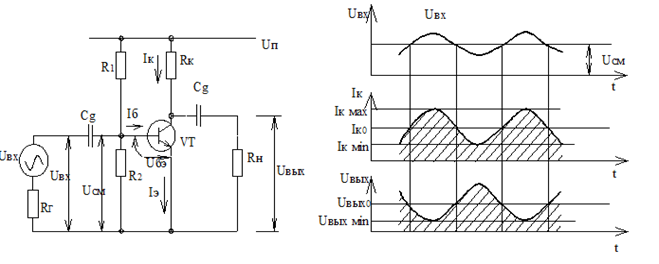
\includegraphics[width=0.8\textwidth]{20_OE.png}
\caption{Схема включения транзистора с общим эмиттером и временная диаграмма его работы}
\label{fig:20_OE}
\end{figure}

При отсутствии входного сигнала выходной ток и выходное напряжение постоянны: Ik = Ik0 и Uk = Uk0.

При поступлении на вход сигнала Uвх он усиливается в Ku раз и снимается с выхода в противофазе по отношению к входному сигналу.

Для усилителя с ОЭ Rвх = $R1 \mid\mid R2 \mid\mid$ Rвх.э ,где Rвх.э = $\beta$Rвх.б. Обычно $R1 \mid\mid R2 \geq (2 \div 5)$Rвх.э ,где Rвх.э не превышает $1 \geq 3$ кОм.

Коэффициент усиления по току $K_I = \beta \dfrac{R_K  \mid\mid R_H}{R_H}$

Таким образом, каскад с ОЭ имеет большой коэффициент усиления по току, который  при Rk>>Rн стремится к $\beta$.

Коэффициент усиления по напряжению $K_U = \beta \dfrac{R_K  \mid\mid R_H}{R_\text{Г} + R_\text{вхб}}$

Коэффициент усиления Ku возрастает с увеличением $\beta$ и $R_H$. Обычно $K_U \approx 10 \div 100$ и выше.

Коэффициент усиления по мощности Kp = Ku * Ki составляет (0,2 --- 5)*$10^3$.

Выходное сопротивление каскада с ОЭ Rвых = $R_K \mid\mid r_\text{КЭ}$. Обычно $r_\text{КЭ} >> R_K$ и $R_\text{вых} \approx R_K$.

Усилительный каскад с ОЭ осуществляет поворот по фазе на 1800 выходного напряжения относительно входного.

Основные режимы работы усилителя. В зависимости от величины смещения на базе транзистора Uсм различают следующие режимы работы усилителя: A, B, AB, C, D.

\subsection*{Класс A}

Режим A характеризуется выбором рабочей точки на линейном участке входной характеристики рисунке ниже. В исходном состоянии транзистор открыт напряжением смещения Uсм и в цепи коллектора протекает ток Iко. При поступлении входного сигнала на выходе усилителя появляется выходной сигнал в противофазе по отношению ко входному.

Режим А характерен тем, что форма выходного сигнала Uвых(t) повторяет форму входного сигнала Uвх(t) за счет работы транзистора в активной зоне без захода в область насыщения и отсечки. Режим характеризуется минимальными нелинейными искажениями.
В то же время работа усилителя в режиме А характеризуется низким КПД, который теоретически не может превышать 0,5, что объясняется постоянным током Iко вне зависимости от наличия или отсутствия входного сигнала. Поэтому такой режим используется только в маломощных каскадах, в которых необходимо иметь минимальные нелинейные искажения.

\begin{figure}[H]
\centering
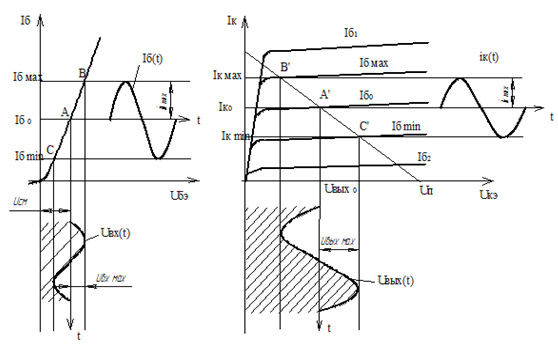
\includegraphics[width=0.6\textwidth]{20_GAA.png}
\caption{Входная и выходная характеристика при работе в классе A}
\label{fig:20_GAA}
\end{figure}

Графоаналитический метод расчета усилителя. По графикам можно определить:

Коэффициент усиления по току $K_I = \dfrac{I_{Kmax}}{I_{bmax}}$

Коэффициент усиления по напряжению $K_U = \dfrac{U_{out.max}}{U_{in.max}}$

Коэффициент усиления по мощности $K_P = K_U K_I$

\subsection*{Класс B}

Режим В характеризуется тем, что напряжение смещения Uсм=0, а следовательно, рабочая точка выбирается в самом начале входной характеристики. Особенностью режима В является то, что при отсутствии входного сигнала отсутствуют базовые и коллекторные токи. 
При поступлении входного сигнала ток в коллекторе имеет пульсирующий характер и протекает в течение половины периода. Режим В характеризуется высоким КПД, который может достигать 70\%, однако выходной сигнал сильно искажается. Поэтому такой режим применяется только в двухтактных усилителях.

\begin{figure}[H]
\centering
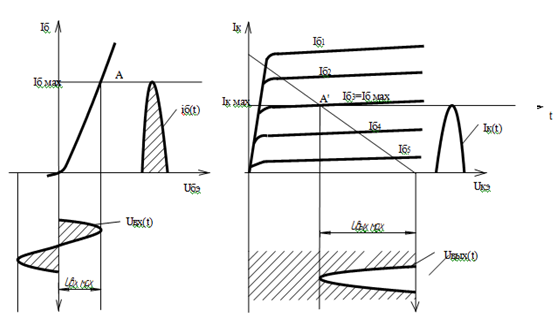
\includegraphics[width=0.6\textwidth]{20_GAB.png}
\caption{Входная и выходная характеристика при работе в классе B}
\label{fig:20_GAB}
\end{figure}

\subsection*{Класс AB}

Режим АВ занимает промежуточное положение между режимами А и В. Он характеризуется небольшим напряжением смещения Uсм и меньшими нелинейными искажениями по сравнению с режимом В. Режим АВ используется в высококачественных двухтактных усилителях мощности.

\subsection*{Класс C}

Режим С характеризуется тем, что рабочая точка на входной характеристике сдвинута влево от начала координат. Следовательно, более половины периода транзистор находится в закрытом состоянии. Режим С характеризуется высоким КПД, большими нелинейными искажениями и применяется в генераторах частоты.

\subsection*{Класс D}

Режим D характеризуется тем, что усилительный элемент может находиться в открытом  (режим насыщения) либо в закрытом (режим отсечки) состояниях. В режиме насыщения базовый ток $I_\text{Б} = \dfrac{I_K\gamma}{\beta}$, где $\gamma$ --- коэффициент насыщения транзистора, который принимается равным 1,5 --- 2.

Таким образом, ток в выходной цепи может принимать только два значения: Ik.max = Iнас. и I k.min $\approx$ 0. Скорость перехода из одного состояния в другое характеризует быстродействие усилительного элемента. Обычно U нас. < 1B, поэтому КПД такого усилительного каскада близок к 1.

Режим работы D, который называют еще ключевым режимом, применяется в импульсных схемах.

\begin{figure}[H]
\centering
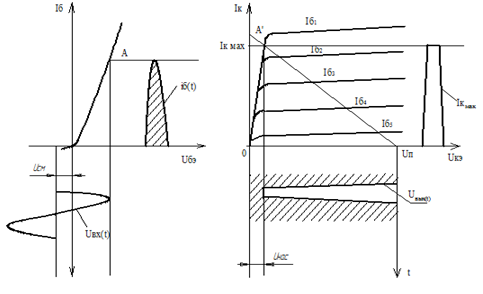
\includegraphics[width=0.6\textwidth]{20_GAD.png}
\caption{Входная и выходная характеристика при работе в классе D}
\label{fig:20_GAD}
\end{figure}

\end{document}